%% 
%% Copyright 2019-2024 Elsevier Ltd
%% 
%% Version 2.4
%% 
%% This file is part of the 'CAS Bundle'.
%% --------------------------------------
%% 
%% It may be distributed under the conditions of the LaTeX Project Public
%% License, either version 1.2 of this license or (at your option) any
%% later version.  The latest version of this license is in
%%    http://www.latex-project.org/lppl.txt
%% and version 1.2 or later is part of all distributions of LaTeX
%% version 1999/12/01 or later.
%% 
%% The list of all files belonging to the 'CAS Bundle' is
%% given in the file `manifest.txt'.
%% 
%% Template article for cas-sc documentclass for 
%% single column output.

%\documentclass[a4paper,fleqn,longmktitle]{cas-sc}
\documentclass[a4paper,fleqn]{cas-sc}

\usepackage[utf8]{inputenc}

%\usepackage[numbers]{natbib}
%\usepackage[authoryear]{natbib}
\usepackage[export]{adjustbox}
\usepackage[authoryear,longnamesfirst]{natbib}
\usepackage{tabularx}
\usepackage{subcaption}
\usepackage{tikz}
\usepackage{pgfplots}

%%%Author macros
\def\tsc#1{\csdef{#1}{\textsc{\lowercase{#1}}\xspace}}
\tsc{WGM}
\tsc{QE}
\tsc{EP}
\tsc{PMS}
\tsc{BEC}
\tsc{DE}
%%%

\pgfplotstableread{
	Participant Evaluation
	1 90.00
	2 95.00
	3 72.50
	4 60.00
	5 85.00
	6 67.50
	7 92.50
	8 67.50
	9 82.50
	10 85.00
	11 92.50
	12 87.50
}\susdata

\widowpenalty10000
\clubpenalty10000

% Valores calculados
\newcommand{\average}{81.46}
\newcommand{\stdev}{11.65}

\pgfmathsetmacro{\upperlimit}{\average+\stdev}
\pgfmathsetmacro{\lowerlimit}{\average-\stdev}


\newcommand{\utequrl}{https://www.uteq.edu.ec} % Define the URL macro

\begin{document}
	\let\WriteBookmarks\relax
	\def\floatpagepagefraction{1}
	\def\textpagefraction{.001}
	\shorttitle{Torddis: Detecting Distractions in Children's Academic Activities}
	\shortauthors{G. Guerrero-Ulloa et~al.}
	%\begin{frontmatter}
	
	\title [mode = title]{Torddis: A Real-Time IoT System for Detecting Distractions in Children's Home-Based  Academic Activities}                        
	\tnotemark[1]
	
	%\tnotetext[2]{The second title footnote which is a longer text matter to fill through the whole text width and overflow into another line in the footnotes area of the first page.}
	
	
	\author[1]{Gleiston Guerrero-Ulloa}[type=editor,orcid=000-0001-5990-2357,style=spanish]
	\ead{gguerrero@uteq.edu.ec}
	\ead[url]{\utequrl}
	
	\credit{Data curation, Methodology, Resources, Supervision, Validation, Visualization, Writing -- original draft, Writing -- review and editing,}
	
	\affiliation[1]{organization={Faculty of Engineering Sciences, State Technical University of Quevedo},
		addressline={Central Campus, Quito Avenue km. 1 1/2, on the way to Santo Domingo de los Tsáchilas}, 
		city={Quevedo},
		postcode={120301}, 
		state={Los Ríos},
		country={Ecuador}
	}
	
	\author[1]{Carlos Almeida-Dueñas}[type=editor,orcid=0000-0002-0959-922X,style=spanish]
	\ead{carlos.almeida2017@uteq.edu.ec}
	\ead[URL]{\utequrl}
	
	\credit{Conceptualization, Data curation, Formal analysis, Investigation, Software, Visualization}
	
	\author[1]{John Plazarte-Suárez}[orcid=0000-0001-5488-9982,style=spanish]
	%\fnmark[2]
	\ead{john.plazarte2017@uteq.edu.ec}
	\ead[URL]{\utequrl}
	
	\credit{Conceptualization, Data curation, Formal analysis, Investigation, Software, Visualization}
	
	\author[1]{Orlando Erazo-Moreta}[type=editor,orcid=0000-0001-5642-9920,
	style=spanish]
	%\fnmark[2]
	\ead{oerazo@uteq.edu.ec}
	\ead[URL]{\utequrl}
	
	\credit{Conceptualization, Data curation, Supervision, Validation, Visualization, Writing -- review and editing}
	
	\author[2]{Carlos Rodríguez-Domínguez}[
	orcid=0000-0001-5626-3115,
	style=spanish,
	%role=Supervisor and Validator
	]
	\cormark[1]
	\ead{carlosrodriguez@ugr.es}
	\ead[URL]{https://lsi.ugr.es/informacion/directorio-personal/carlos-rodriguez-dominguez}
	
	\credit{Data curation, Supervision, Validation, Visualization, Writing -- review and editing}
	
	\author[2]{Miguel J. Hornos}[orcid=0000-0001-5722-9816,style=spanish]
	%\fnmark[1,3]
	\ead{mhornos@ugr.es}
	\ead[URL]{https://lsi.ugr.es/informacion/directorio-personal/miguel-juan-hornos-barranco}
	
	\affiliation[2]{organization={Software Engineering Department, University of Granada},
		addressline={Calle Periodista Daniel Saucedo Aranda s/n}, 
		postcode={18071}, 
		postcodesep={}, 
		city={Granada},
		country={Spain}
	}
	
	\credit{Data curation, Supervision, Validation, Visualization, Writing -- review and editing}
	
	\cortext[cor1]{Corresponding author}
	%\cortext[cor2]{Principal corresponding author}
	
	%\nonumnote{Torddis is an innovative IoT system designed to monitor and improve student concentration at home, providing tutors with tools to detect distractions and maintain focus on school tasks.}
	
	%\fntext[fn1]{This document is the result of research conducted as part of teaching activities at the Technical State University of Quevedo, applying the findings from the Ph.D. thesis at the University of Granada.}
	
	\begin{abstract}
		Torddis es un sistema innovador diseñado para mitigar los efectos del ausentismo parental en el rendimiento académico mediante el uso de tecnologías de Inteligencia Artificial (IA) e Internet de las Cosas (IoT). El sistema monitorea en tiempo real las distracciones de los estudiantes en entornos domésticos, detectando expresiones faciales indicativas de distracción, objetos no autorizados y signos de somnolencia. Desarrollado utilizando la metodología TDDM4IoTS, Torddis integra una aplicación móvil con un dispositivo IoT para ofrecer a los tutores una herramienta práctica y eficiente para supervisar las actividades académicas en el hogar. Las evaluaciones de usabilidad realizadas por los tutores arrojaron una alta puntuación en la escala de usabilidad del sistema (SUS) del 81.46\%, lo que subraya la efectividad del sistema en mejorar la concentración de los estudiantes y proporcionar información valiosa para los padres. Aunque el sistema ha demostrado un potencial significativo, se han señalado recomendaciones para mejorar la calidad de la cámara. Torddis aspira a tener un impacto sustancial en la educación, sirviendo como un aliado robusto en el proceso de aprendizaje y ofreciendo prometedoras vías para futuros avances tecnológicos.
	\end{abstract}
	
	\begin{graphicalabstract}
		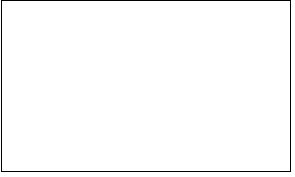
\includegraphics{figs/cas-grabs.pdf}
	\end{graphicalabstract}
	
	\begin{highlights}
		\item \textbf{Integración de Inteligencia Artificial e IoT:} Torddis utiliza tecnologías de IA e IoT para monitorizar en tiempo real las distracciones de los estudiantes en el hogar. El sistema identifica expresiones faciales indicativas de distracción, objetos no autorizados y signos de somnolencia, proporcionando una herramienta accesible y eficiente para la supervisión académica.
		\item \textbf{Metodología TDDM4IoTS:} Desarrollado siguiendo la metodología TDDM4IoTS, Torddis asegura la integración efectiva de una aplicación móvil y un dispositivo IoT, mejorando la supervisión académica y la concentración de los estudiantes. Esta metodología facilita el análisis del comportamiento de los niños mientras realizan tareas escolares de forma independiente en el hogar.
		\item \textbf{Evaluación de Usabilidad:} La usabilidad del sistema fue evaluada positivamente por los tutores, logrando una notable puntuación del 81.46\% en la escala de usabilidad del sistema (SUS). Esto resalta los beneficios del sistema para mejorar la concentración de los estudiantes y brindar apoyo informativo a los padres.
		\item \textbf{Alertas Visuales y Auditivas:} Los tutores enfatizaron la importancia de las alertas visuales y auditivas para mantener la atención de los estudiantes. El sistema incluye funciones que permiten la personalización de mensajes de audio y visuales, ayudando a mantener el enfoque de los niños durante las actividades académicas.
		\item \textbf{Impacto en la Educación:} Torddis promete un impacto significativo en la educación, posicionándose como un fuerte aliado en el aprendizaje y ofreciendo oportunidades para un mayor desarrollo. La integración de tecnologías avanzadas para la detección y respuesta en tiempo real a las distracciones subraya la relevancia de la innovación tecnológica en el ámbito educativo.
	\end{highlights}
	
	\begin{keywords}
		Internet of Things \sep
		Artificial Intelligence \sep
		Computer Vision \sep
		Distraction Monitoring \sep
		Student Concentration
	\end{keywords}
	
	\maketitle
	
	\section{Introducción}
	\label{seccion:Uno}
	Durante la última década, los estilos de vida acelerados y el aumento de la carga laboral han llevado a un incremento en el ausentismo parental durante las horas reservadas para las actividades de los estudiantes de primaria, lo cual ha resaltado la necesidad de soluciones tecnológicas que puedan suplir esta carencia de supervisión \cite{Abdul-Aziz2022}.
	
	Esta ausencia y falta de apoyo han demostrado afectar directamente el rendimiento académico de los jóvenes estudiantes. Los docentes han observado una disminución en los indicadores de rendimiento y disciplina, lo cual podría impactar negativamente la autoestima de los estudiantes y otros aspectos psicosociales. Además, la literatura sugiere que el apoyo emocional en el hogar es un pilar esencial para que los niños se concentren en sus estudios \citep{Abdul-Aziz2022}.
	
	La interferencia emocional influye no solo en el éxito educativo, sino que también impacta de manera significativa en todos los aspectos de la vida de los estudiantes \citep{Ake2023}. En este contexto, un entorno familiar que promueva la comunicación positiva y la interacción genuina puede mejorar el bienestar y las habilidades sociales de los estudiantes \citep{Navarro2024}. Sin embargo, para abordar de manera efectiva los desafíos asociados con la atención y la regulación emocional, es fundamental incorporar herramientas tecnológicas que integren Inteligencia Artificial (IA) e Internet de las Cosas (IoT). Estas tecnologías permiten monitorizar y medir las distracciones de los niños, proporcionando datos cruciales para la toma de decisiones orientadas a mejorar la atención y el aprendizaje \citep{Alvear-Puertas2017,Berrezueta-Guzman2021}.
	
	El uso de herramientas tecnológicas basadas en IA e IoT no solo contribuye al mejoramiento del rendimiento académico, sino que también fomenta habilidades de autorregulación en los estudiantes, esenciales para su desarrollo cognitivo y socioemocional \citep{Mohamed201862}. La retroalimentación que ofrecen estas tecnologías ayuda a los estudiantes a identificar sus distracciones y tomar acciones correctivas, lo que refuerza su capacidad para gestionar el tiempo y concentrarse en sus actividades. De esta manera, las herramientas tecnológicas se presentan como un recurso valioso para complementar la influencia positiva del entorno familiar y potenciar el aprendizaje autorregulado, creando un enfoque integral que abarca tanto el ámbito educativo como el personal \cite{Thinyane2016AUG}.
	
	La concentración de los estudiantes es un factor crucial que determina su capacidad para aprender y aplicar los conocimientos impartidos por los docentes. En un estudio realizado por \cite{Terraza2022}, se propone un sistema para monitorizar la atención de los estudiantes en un entorno de aprendizaje en línea utilizando algoritmos de visión por computadora. Los autores utilizan una Red Neuronal Recurrente (RNN) para identificar puntos de referencia faciales, que detectan si un estudiante mantiene una posición frontal hacia el dispositivo utilizado para asistir a una clase en línea. Su estudio resalta algunas limitaciones presentes en las propuestas actuales.
	
	Por otro lado, el trabajo de \cite{Berrezueta-Guzman2021} presenta un sistema robótico diseñado para interactuar con niños diagnosticados con Trastorno por Déficit de Atención e Hiperactividad (TDAH) para ayudarles a corregir hábitos poco saludables y comportamientos inapropiados asociados con el TDAH. Este sistema está orientado a niños diagnosticados con TDAH; sin embargo, a pesar de sus aspectos prometedores, cuando se aplica de manera general, puede perturbar a los niños sin tales condiciones. Además, este sistema carece de funciones de notificación, alerta o alarma para informar a sus tutores.
	
	En un esfuerzo por incluir la participación del tutor para mejorar el bienestar emocional de los niños, se introduce Torddis\footnote{Del latín \textbf{Tor}queo \textbf{d}iscerno \textbf{dis}cipulus'', que significa ``detección de desviación o cambio en la atención del estudiante.''}, como una solución que utiliza los avances tecnológicos para monitorizar el comportamiento de los estudiantes mientras realizan tareas escolares de forma independiente en sus hogares e informa a los tutores sobre cualquier desarrollo, para que puedan asegurar a sus hijos que no están solos. Además, Torddis está habilitado para reproducir sonidos que pueden ser mensajes personalizados de acuerdo con las preferencias de los usuarios.
	
	Para lograr sus objetivos, Torddis emplea algoritmos avanzados de visión por computadora y técnicas de aprendizaje profundo. El sistema incluye una aplicación móvil para tutores y un dispositivo IoT que facilita el análisis del comportamiento de los niños mientras realizan tareas escolares por su cuenta. Desarrollado utilizando la metodología TDDM4IoTS \citep{Guerrero-Ulloa2020TDDM4IoTS}, Torddis se destaca por su enfoque holístico. Permite a los tutores monitorizar y responder en tiempo real a signos de inatención. Las características clave incluyen la capacidad de detectar expresiones faciales que representan emociones fundamentales e identificar signos de somnolencia o el uso inadecuado de objetos durante las actividades educativas. Esta funcionalidad permite a los tutores alentar a sus hijos a mantener la concentración, utilizando tanto estímulos visuales como auditivos como motivadores \citep{Al-Gburi2023,Enadula2021,Terraza2022}.
	
	El sistema Torddis está diseñado para reforzar habilidades metacognitivas, como la gestión del tiempo y la concentración, esenciales en el aprendizaje moderno y en el contexto del aprendizaje autónomo. Su enfoque en la supervisión proactiva responde a la necesidad de apoyar a los niños durante una etapa crítica de desarrollo, proporcionando a los tutores una herramienta valiosa que complementa la supervisión tradicional en el hogar y contribuye a mejorar los resultados educativos de esta población.
	
	Este artículo está organizado en secciones que cubren diferentes aspectos de la implementación de la propuesta actual. La Sección \ref{seccion:Dos} se plantea la dimensión pedagógica del sistema TORDDIS. En La Sección \ref{seccion:Tres} revisa trabajos relacionados publicados en revistas internacionales de prestigio durante los últimos diez años. Estos trabajos están indexados en bases de datos como Web of Science (WoS), IEEE Xplore, ACM Digital Library y PubMed. La sección \ref{seccion:Cuatro} describe los materiales y métodos utilizados a lo largo del desarrollo y los procesos de evaluación del sistema. La Sección \ref{seccion:Cinco} presenta los principales resultados y discusión, y la Sección \ref{seccion:Seis} expone las conclusiones.
	
	\section{Dimensión Pedagógica de Torddis}
	\label{seccion:Dos}	
	Torddis, además de ofrecer soluciones tecnológicas para la monitorización de la concentración de los estudiantes, aborda la importancia del aprendizaje autónomo y la autorregulación, aspectos fundamentales en el desarrollo académico y personal de los niños.
	
	La autorregulación, entendida como la capacidad de los estudiantes para gestionar y evaluar su propio proceso de aprendizaje, se convierte en una competencia esencial en el aprendizaje moderno. Diversas investigaciones, que abarcan desde la implementación de lenguajes de programación visual en la educación primaria \citep{SaezLopez2016Visual} hasta la incorporación de metodologías activas en el aula \citep{Mohamed2018Implementing}, resaltan que los entornos tecnológicos y las estrategias pedagógicas pueden promover significativamente la autorregulación en los estudiantes.
	
	Estos enfoques permiten a los niños interactuar de forma autónoma y reflexiva, generando hábitos que fortalecen su capacidad para mantener la concentración y gestionar su tiempo y sus recursos de manera efectiva. En este contexto, Torddis se presenta no solo como una herramienta de monitorización, sino como un aliado pedagógico que contribuye al desarrollo de habilidades de autorregulación y refuerza el rol del tutor o profesor en el proceso de aprendizaje.
	
	\subsection{Importancia de la autorregulación en el aprendizaje}
	El desarrollo de la autorregulación en el aprendizaje resulta fundamental para la autonomía académica, ya que permite a los estudiantes tomar control sobre su propio proceso de aprendizaje, estableciendo metas, evaluando sus avances y ajustando sus estrategias. La investigación de \cite{Taber2024Developing} ejemplifica cómo la autorregulación es esencial en disciplinas que demandan habilidades de gestión autónoma, permitiendo a los estudiantes monitorizar y mejorar continuamente su rendimiento.
	
	Asimismo, los entornos educativos pueden fomentar esta competencia mediante metodologías activas y el uso de tecnologías. Por ejemplo, el uso de lenguajes de programación visual, como Scratch, en la educación básica ayuda a los estudiantes a experimentar y tomar decisiones, desarrollando así habilidades de autorregulación a través de la exploración y el control personal de sus actividades de aprendizaje. El aula invertida apoyada por sistemas de tutoría inteligente, descrito en el trabajo de \cite{Mohamed2018Implementing} permite a los estudiantes trabajar de forma independiente fuera del aula y recibir retroalimentación inmediata, promoviendo un proceso de aprendizaje autorregulado y adaptativo.
	
	Finalmente, el uso de dinámicas de juego colaborativo, como  exploran \cite{Echeverria2011AFramework} contribuye al desarrollo de competencias de autorregulación en un entorno lúdico. Estas experiencias, al involucrar al estudiante en la toma de decisiones y el manejo de objetivos, consolidan habilidades de autocontrol y manejo de tiempo esenciales en el aprendizaje autónomo.
	
	Estas investigaciones destacan que el desarrollo de la autorregulación mediante enfoques tecnológicos y pedagógicos no solo optimiza el aprendizaje autónomo, sino que también prepara a los estudiantes para enfrentar de forma reflexiva y adaptativa los retos de su proceso educativo.
	
	\subsection{Torddis y su contribución a la supervisión del aprendizaje autónomo en el hogar}
	
	El sistema Torddis está diseñado para apoyar el aprendizaje autónomo en los estudiantes a través de herramientas tecnológicas que permiten la supervisión y la monitorización en tiempo real de la concentración durante sus actividades académicas en el hogar. Mediante el análisis de expresiones faciales, la detección de objetos y el reconocimiento de estados de somnolencia, el sistema ayuda a los estudiantes a mantener el enfoque en sus tareas escolares, permitiéndoles desarrollar habilidades esenciales de autorregulación como la atención sostenida, la gestión del tiempo y el autocontrol.
	
	Una característica clave de Torddis es su capacidad para detectar distracciones y emitir alertas visuales y sonoras, brindando a los estudiantes una retroalimentación inmediata que los ayuda a redirigir su atención hacia las actividades académicas. Esta retroalimentación en tiempo real refuerza el proceso de autorreflexión y autoevaluación, aspectos cruciales en la autorregulación del aprendizaje. Además, al incorporar a los tutores en el proceso, Torddis establece un entorno de aprendizaje colaborativo donde los padres pueden observar y analizar los patrones de comportamiento de sus hijos, lo que permite una intervención oportuna en caso de que se identifiquen barreras para el aprendizaje.
	
	La capacidad de Torddis para registrar y visualizar datos históricos de las distracciones de los estudiantes y otros parámetros relevantes también permite un seguimiento constante y la identificación de áreas específicas en las que el estudiante podría mejorar su autorregulación. Este enfoque integral no solo optimiza el tiempo y esfuerzo del estudiante, sino que también proporciona a los tutores una herramienta confiable para apoyar el proceso de aprendizaje en ausencia de supervisión constante, promoviendo una educación que fomente la autonomía y la autogestión en el estudiante.
	
	\subsection{Relación de Torddis con las competencias digitales}
	Torddis se presenta como una herramienta educativa que promueve activamente el desarrollo de competencias digitales entre los estudiantes. En la era de la digitalización, los estudiantes requieren habilidades que les permitan interactuar eficazmente con herramientas tecnológicas para maximizar sus oportunidades de aprendizaje y, al mismo tiempo, adquirir habilidades críticas para el futuro. El sistema apoya este desarrollo al facilitar un entorno en el cual los estudiantes pueden participar en actividades interactivas y autónomas, permitiéndoles mejorar sus competencias en la resolución de problemas y en el uso efectivo de la tecnología educativa.
	
	Implementaciones como el aula invertida, donde los estudiantes acceden a contenido digital fuera del horario de clases y emplean las horas presenciales para actividades prácticas, han demostrado ser eficaces en el aumento de la motivación y del compromiso del estudiante al situarlos en el centro del proceso de aprendizaje, promoviendo un ambiente de colaboración y un aprendizaje autodirigido, que son componentes esenciales de las competencias digitales \citep{Mohamed2018Implementing}. Además, estudios en entornos de aprendizaje colaborativo evidencian que el uso de juegos digitales y plataformas de aprendizaje programado contribuyen al desarrollo de habilidades digitales y colaborativas al proporcionar escenarios de aprendizaje basados en la interacción con herramientas digitales \citep{Echeverria2011AFramework}, algo que Torddis también facilita a través de su diseño orientado a la interacción y la supervisión en tiempo real.
	
	\cite{Coffman2024Developing} mencionan que en el ámbito de la educación en enfermería, la autorregulación ha sido una estrategia fundamental para fomentar la autodisciplina y el uso efectivo de tecnologías digitales en el aprendizaje, demostrando que los estudiantes mejoran su rendimiento académico y su adaptabilidad a entornos clínicos y digitales al incorporar estrategias de autorregulación que Torddis puede fomentar desde edades tempranas mediante supervisión y retroalimentación constante. Por lo tanto, Torddis se alinea con las mejores prácticas de pedagogía moderna, apoyando un aprendizaje autónomo y digitalmente competente, necesario para responder a las demandas del siglo XXI.
	
	\section{Related Works}
	\label{seccion:Tres}
	La literatura sobre el uso de tecnologías para la detección y corrección de distracciones en estudiantes es limitada, especialmente en lo que respecta a la integración de tecnologías IoT con fines pedagógicos. Los estudios previos han abordado aplicaciones tecnológicas en la monitorización de niños, pero pocos han explorado cómo estas tecnologías pueden ser utilizadas para proporcionar retroalimentación inmediata que fomente la autorregulación del aprendizaje y mejore los resultados educativos en contextos no formales.El proceso de revisión del estado del arte siguió la metodología descrita en el esquema de la Figura \ref{fig:LRS}.
	
	\begin{figure}[h]
		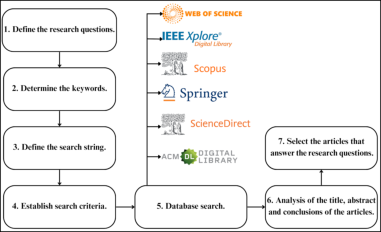
\includegraphics[width=\textwidth]{figs/Figure_1}
		\caption{Literature Review Scheme.}
		\label{fig:LRS}
	\end{figure}   
	
	\subsection{Research Questions}
	Este artículo explora el tema crítico de la detección de distracciones en los estudiantes mientras realizan tareas escolares de forma independiente. Con el aumento de las herramientas digitales de educación y la necesidad de estrategias de aprendizaje efectivas, comprender cómo las distracciones afectan el rendimiento estudiantil se ha vuelto fundamental. Las siguientes preguntas de investigación tienen como objetivo guiar una revisión exhaustiva de los trabajos relacionados e informar el desarrollo de soluciones tecnológicas que mejoren la concentración y los resultados educativos de los niños. Estas preguntas ayudarán a identificar los métodos y tecnologías más efectivos para monitorizar y mitigar las distracciones durante las actividades educativas.
	
	\begin{itemize}
		\item ¿Cuáles son los parámetros de distracción que deberían monitorizarse en los niños durante la realización de sus tareas escolares?
		\item ¿Qué modelos computacionales son adecuados para detectar el comportamiento de los niños mientras realizan tareas escolares?
		\item ¿Qué algoritmos enfocados en la detección de distracciones podrían ser utilizados en el desarrollo de la propuesta?
		\item ¿Qué tecnologías de hardware y software podrían emplearse para desarrollar un dispositivo prototipo que apoye la concentración de los niños durante las actividades escolares?
	\end{itemize}
	%\unskip
	
	\subsection{Estrategias de Búsqueda}
	Una vez definidas las preguntas de investigación, se seleccionaron las palabras clave relevantes para recuperar trabajos publicados en las principales bases de datos científicas más pertinentes para este campo de investigación. Estas palabras clave se utilizaron para formar la cadena de búsqueda, la cual fue adaptada específicamente para cada base de datos científica seleccionada. La cadena de búsqueda utilizada fue: ("distracción") AND ("niño" OR "niños" OR "estudiante" OR "tarea escolar" OR "deberes") AND ("reconocimiento de objetos" OR "reconocimiento facial" OR "reconocimiento de gestos").
	
	Las bases de datos utilizadas incluyeron ACM, IEEE Xplorer, PubMed, Scopus y Web of Science. Además, se empleó Google Scholar para ampliar los resultados y así minimizar la posibilidad de excluir documentos importantes como trabajos relacionados. La Tabla \ref{tab:Results} muestra la búsqueda inicial en estas bases de datos y en Google Scholar. Tras un análisis individual de los documentos encontrados en las bases de datos, se consideró que el 82\% de ellos eran relevantes. En contraste, de los resultados del motor de búsqueda académico, se revisaron los primeros 500 resultados en orden de relevancia, con 6 (y duplicados 16) de los primeros 300 considerados pertinentes. Los siguientes 200 resultados no estaban relacionados con las preguntas de investigación de este estudio, lo que llevó a asumir que no se encontrarían más documentos relevantes.
	
	\begin{table}[H] 
		\caption{Resultados de la búsqueda de trabajos relacionados.\label{tab:Results}}
		\begin{tabularx}{0.90\textwidth}{>{\centering\arraybackslash}X >{\centering\arraybackslash}X >{\centering\arraybackslash}X >{\centering\arraybackslash}X >{\centering\arraybackslash}X}
			\toprule
			\textbf{Base de Datos/Motor de Búsqueda}	& \textbf{Resultados Preliminares} & \textbf{Duplicados} & \textbf{Análisis de Título y Resumen} & \textbf{Resultados Finales}\\
			\midrule
			ACM 			& 	1 		& 	0 	& 	1	&	1\\
			IEEE Xplorer	& 	3		&  	0 	& 	2	&	2\\
			PubMed			&  	1 		& 	0 	& 	0	&	0\\
			Scopus			&  	22 		& 	3 	& 	19	&	15\\
			Web of Science	&  	8 		& 	6 	& 	2	&	2\\
			Google Scholar	&  	15,400 (primeros 500) 	& 	19 	& 	16	&	6\\
			\bottomrule
		\end{tabularx}
	\end{table}
	
	\subsection{Análisis de la Literatura}			
	En la literatura científica sobre tecnologías aplicadas a los sectores de la educación y el cuidado infantil, existen diversos enfoques centrados en el uso de IA, IoT y técnicas de visión por computadora para mejorar el aprendizaje y la monitorización del comportamiento. Investigaciones de \cite{Pelc2006}, \cite{Albrecht2014}, \cite{Warren2015Brief}, \cite{Washington2016AWereable}, \cite{Akter2021}, \cite{Berrezueta-Guzman2021}, y \cite{VilliersRader2021} exploran aplicaciones que van desde el diagnóstico temprano del trastorno del espectro autista hasta la mejora en el reconocimiento de emociones en niños con trastornos de déficit de atención. Todos estos estudios utilizan tecnologías avanzadas para analizar y responder a comportamientos específicos de los niños en entornos controlados o cotidianos, enfocándose en detectar y responder a las necesidades particulares de los niños mediante algoritmos de IA y dispositivos conectados.
	
	Aunque estos esfuerzos de investigación comparten fundamentos tecnológicos, sus objetivos y metodologías específicas varían significativamente. \cite{Pelc2006} se enfoca en reconocer emociones en niños con TDAH utilizando fotografías validadas, mientras que \cite{Albrecht2014} investigan las estrategias de búsqueda visual en niños con TEA. Por otro lado, \cite{Akter2021} emplean el aprendizaje por transferencia para diagnosticar el trastorno del espectro autista (TEA) mediante el reconocimiento facial.
	
	\cite{Berrezueta-Guzman2021} evalúan el uso de un asistente robótico para apoyar las actividades escolares de niños con TDAH, y \cite{VilliersRader2021} examinan cómo los gestos pueden dirigir la atención hacia las relaciones entre palabras y objetos en niños con TEA. Cada uno de estos estudios proporciona una perspectiva única sobre cómo las tecnologías pueden adaptarse para abordar diferentes aspectos del aprendizaje y la interacción social.
	
	Estudios adicionales de \cite{James2019}, \cite{Hachad2020}, \cite{Enadula2021}, \cite{Ozdamli2022}, \cite{Kulkarni2023}, \cite{Narkhede2023}, \cite{Farsani2020}, \cite{Boumiza2017}, \cite{Muller2018ArchnSmile}, \cite{DaCosta2023}, y \cite{Kumar2024Zoom} ilustran una clara tendencia hacia el uso del reconocimiento facial y la IA para resolver diversos problemas en entornos educativos y de seguridad. Cada uno de ellos contribuye a un panorama tecnológico más amplio que mejora la interacción y la seguridad de los estudiantes.
	
	\cite{James2019} y \cite{Hachad2020} utilizan el reconocimiento facial en la educación en diferentes contextos. James y Nettikadan \cite{James2019} monitorean la seguridad de los estudiantes en autobuses escolares, mientras que \cite{Hachad2020} gestionan la asistencia de los estudiantes en las aulas. Ambos aprovechan tecnologías como OpenCV y algoritmos de reconocimiento facial para abordar la seguridad durante el transporte y la eficiencia en la toma de asistencia, demostrando la versatilidad del reconocimiento facial en diferentes entornos educativos.
	
	\cite{Enadula2021} y \cite{Ozdamli2022} exploran el reconocimiento de emociones en estudiantes en la educación en línea y los exámenes a distancia, respectivamente. Ambos emplean tecnologías de visión por computadora para analizar expresiones faciales, y \cite{Ozdamli2022} también incorporan la detección de trampas, destacando el potencial del reconocimiento facial para mejorar la interacción de los estudiantes en entornos virtuales. Mientras que \cite{Muller2018ArchnSmile} utilizan la inteligencia artificial para el reconocimiento de emociones para controlar Arch'n'Smile, un juego de tipo "jump-and-run" diseñado para que los niños jueguen durante viajes en coche, enfocado en el entretenimiento infantil.
	
	\cite{Kulkarni2023}, \cite{Narkhede2023}, \cite{Farsani2020}, y \cite{Kumar2024Zoom} se centran en diferentes aplicaciones del reconocimiento facial para el seguimiento de la asistencia y la atención de los estudiantes. Mientras que \cite{Kulkarni2023} y \cite{Narkhede2023} registran la asistencia, \cite{Farsani2020} examina cómo los gestos de los docentes afectan la atención visual de los estudiantes, subrayando la utilidad de las tecnologías
	
	avanzadas para mejorar tanto la administración como la experiencia educativa. El sistema propuesto por \cite{Kumar2024Zoom} utiliza tecnologías de detección de imágenes, seguimiento ocular y algoritmos de análisis de datos para mejorar la participación y la atención de los estudiantes.
	
	\cite{Boumiza2017} y \cite{DaCosta2023} utilizan el reconocimiento facial para la tutoría automatizada y la monitorización de los estudiantes en el transporte escolar en ciudades inteligentes, respectivamente. Ambos enfatizan el uso integrado de tecnologías avanzadas para mejorar la seguridad y personalizar el aprendizaje, demostrando cómo el reconocimiento facial puede extenderse más allá del aula hacia soluciones educativas y urbanas más amplias.
	
	Otros estudios de \cite{Riquelme2013}, \cite{Nguyen2019}, y \cite{Argel2023Intellitell} también emplean tecnologías avanzadas en el reconocimiento facial y de gestos para evaluar y mejorar el compromiso de los estudiantes en entornos educativos. Utilizando sistemas como YOLOv3, analizan visualmente las respuestas de los estudiantes durante las sesiones de clase, lo que permite la monitorización en tiempo real y el ajuste dinámico de los métodos de enseñanza para satisfacer mejor las necesidades y los estados emocionales de los estudiantes.
	
	A pesar de las similitudes tecnológicas, los enfoques y objetivos de \cite{Erazo2016Easing}, \cite{Nguyen2019} y \cite{Riquelme2013} difieren significativamente. En su estudio, \cite{Erazo2016Easing} proponen el uso de aplicaciones basadas en gestos sin contacto para facilitar la participación de los estudiantes en clase desde sus ubicaciones físicas. Este enfoque tiene el potencial de aumentar el compromiso, mejorar la presentación del material y crear clases más atractivas e interactivas.
	\cite{Nguyen2019} se centran en la detección de emociones y el desarrollo de la empatía a través de la lectura mediada de literatura infantil para comprender mejor los niveles de atención e interés de los estudiantes. De manera similar, \cite{Argel2023Intellitell} presentan Intellitell, una plataforma web enfocada en la detección de emociones utilizando modelos de aprendizaje automático, desarrollada como una herramienta para analizar y comprender las emociones presentes en historias narrativas.
	
	En contraste, \cite{Riquelme2013} reconocen posturas y gestos para mejorar la adaptabilidad del aprendizaje, evaluando las interacciones físicas de los estudiantes con el contenido presentado para una mayor personalización de la experiencia educativa. \cite{Nguyen2019} crean su propio conjunto de datos para el entrenamiento de modelos, mientras que \cite{Riquelme2013} usan el aprendizaje por transferencia con modelos preentrenados para optimizar su sistema.
	
	Un trabajo notable es presentado por \cite{Campbell2015Using}, el cual consiste en un sistema para monitorizar el comportamiento de los estudiantes en entornos educativos utilizando imágenes multiespectrales para detectar distracciones causadas por dispositivos móviles. No se especifica la edad ni el nivel educativo de los estudiantes. Sin embargo, dado que está diseñado para monitorizar los efectos del uso de dispositivos móviles, no es aplicable para monitorizar a estudiantes de primaria. Además, el sistema no detecta distracciones en momentos específicos, como cuando los estudiantes están haciendo sus tareas. Por otro lado, \cite{Ucar2022Recognizing} presentan un software desarrollado para monitorizar el compromiso de los estudiantes en tiempo real mediante el procesamiento de imágenes, centrado en el reconocimiento facial y la estimación de la postura de la cabeza. Este sistema proporciona retroalimentación en tiempo real para adaptar el flujo del curso según los niveles de compromiso de los estudiantes, mejorando la experiencia de aprendizaje en línea.
	
	Los estudios adicionales proporcionados en este análisis comparten un enfoque común hacia la integración de tecnologías para facilitar la autorregulación del aprendizaje, mejorar la concentración y fomentar el compromiso académico en diversos grupos de estudiantes. El estudio de \cite{Bembich2016Future} se centra en el uso de tecnologías digitales para apoyar el aprendizaje continuo y sin interrupciones en futuros educadores, proporcionando estrategias de autorregulación para gestionar las distracciones y promover la continuidad en el aprendizaje. Por otro lado, \cite{Peters2003Self} examina cómo las tecnologías basadas en entornos hipertextuales pueden mejorar el control volicional y la gestión de distracciones, enfocándose en el aprendizaje digital autónomo de los estudiantes.
	
	De manera similar, \cite{Roberts2020Task} aborda cómo los estudiantes de secundaria utilizan registros digitales de aprendizaje en entornos con dispositivos Chromebook para fomentar la autorregulación, haciendo un seguimiento de su progreso académico y reflexionando sobre sus avances. \cite{Adcroft2018Developing} combina tecnologías con prácticas de manejo del tiempo y mindfulness, enfocándose en ayudar a los estudiantes a mejorar su concentración y autorregulación en sus tareas diarias. Por último, \cite{Salter2014Exploring} presenta un enfoque a nivel escolar que integra tecnologías y plataformas para monitorizar y evaluar el progreso de los estudiantes en el desarrollo de habilidades de autorregulación, destacando un soporte integral para mejorar la experiencia educativa.
	
	trabajos proporcionados abordan, en distintos niveles, la autorregulación, el compromiso académico y las estrategias para mitigar distracciones, pero lo hacen con enfoques específicos y destinatarios diferenciados. "Instructional Designers Conducting Professional Learning Using Social Media" se centra en profesionales que diseñan materiales educativos y cómo utilizan redes sociales para su desarrollo continuo. Aquí, la tecnología se emplea como un medio de colaboración y aprendizaje autorregulado en un contexto profesional. Este enfoque difiere considerablemente de otros trabajos que se enfocan más directamente en los estudiantes, como "Empowering College Students to Decrease Digital Distraction Through the Use of Self-Regulated Learning Strategies", que aborda estrategias específicas para reducir las distracciones digitales en estudiantes universitarios mediante habilidades de autorregulación. Aunque ambos destacan la autorregulación, su enfoque es claramente distinto, ya que el primero se dirige a profesionales y el segundo a estudiantes.
	
	El estudio "The interplay between time perspective, internet use and smartphone in-class multitasking" analiza cómo el uso de dispositivos móviles afecta la atención y el multitasking en entornos educativos, principalmente en adultos y estudiantes universitarios. Comparado con "Smartphone Usage and Studying: Investigating Relationships between Type of Use and Self-Regulatory Skills", que también examina el impacto de los teléfonos inteligentes, el primero adopta un enfoque más psicológico al analizar la percepción del tiempo y su influencia, mientras que el segundo aborda directamente cómo ciertos tipos de uso impactan las habilidades de autorregulación. Estas diferencias reflejan cómo los estudios sobre distracciones digitales divergen en sus metodologías, aunque comparten un objetivo común: comprender y reducir las distracciones para mejorar el rendimiento académico.
	
	Por otro lado, "The impact of synchronous hybrid instruction on students’ engagement in a pharmacotherapy course" ofrece un análisis sobre cómo la enseñanza híbrida sincrónica afecta el compromiso estudiantil, pero su contexto es específico para la educación farmacéutica. Este trabajo, aunque relevante para el estudio del compromiso, no aborda de manera explícita el manejo de distracciones digitales ni estrategias de autorregulación aplicables a menores de edad, diferenciándose así de otros trabajos que tienen un enfoque más amplio.
	
	La comparación entre estos estudios revela que, si bien todos comparten el interés en la mejora del compromiso y la autorregulación, su aplicación y enfoque varían considerablemente. Algunos están dirigidos a adultos y profesionales en contextos muy específicos, mientras que otros buscan influir en estudiantes universitarios mediante estrategias específicas contra la distracción. Sin embargo, la mayoría de estos estudios carece de una solución tecnológica integrada que permita una monitorización en tiempo real de las distracciones y una intervención adaptativa, especialmente para niños.
	
	
	Los estudios analizados comparten el objetivo de utilizar tecnología para mejorar la concentración, la autorregulación y el compromiso académico, aunque presentan diferencias notables en su enfoque y destinatarios. Algunos se orientan a grupos específicos, como futuros maestros o adolescentes en entornos digitales, mientras que otros adoptan un enfoque integral a nivel escolar. La mayoría de estas propuestas, sin embargo, carecen de un componente de monitorización en tiempo real y no emplean tecnologías avanzadas como el reconocimiento facial o de objetos para detectar distracciones con precisión y ofrecer respuestas adaptativas. En general, se centran en la autorregulación del estudiante, dependiendo de su compromiso directo sin incluir una supervisión activa de tutores o padres, lo que limita su capacidad para intervenir en situaciones críticas de distracción.
	
	En contraste, TORDDIS ofrece un enfoque proactivo y personalizado que supera la monitorización pasivo de los sistemas tradicionales. Integrando IoT, visión por computadora e inteligencia artificial, permite a los tutores ejercer un control activo sobre las actividades escolares de los niños, con capacidades de supervisión precisa y alertas visuales y sonoras en tiempo real para intervenir oportunamente. Esta combinación tecnológica no solo ayuda a los estudiantes a mantener la concentración, sino que proporciona a sus tutores herramientas para comprender mejor los patrones de comportamiento y fomentar una experiencia de aprendizaje más comprometida y efectiva. A diferencia de las tecnologías existentes que se enfocan en análisis pasivo, TORDDIS se convierte en un mediador activo que detecta y responde a distracciones, siguiendo los principios del aprendizaje autorregulado \citep{NG201865}. De acuerdo con esta teoría, el rendimiento mejora significativamente cuando los estudiantes reciben retroalimentación inmediata que les permite ajustar sus estrategias de manera oportuna \citep{Taber2024Developing}.
	
	TORDDIS también destaca por su capacidad de abordar la distracción en el hogar, un entorno menos estructurado y más impredecible que el aula tradicional. Mediante el uso de IoT y análisis de comportamiento impulsado por IA, TORDDIS ofrece una monitorización integral que incluye reconocimiento de expresiones faciales, detección de objetos no autorizados y evaluación de actividad. Esta capacidad multidimensional no solo identifica distracciones, sino que actúa proactivamente para redirigir la atención del niño hacia sus tareas, en ausencia de supervisión adulta constante. De este modo, TORDDIS no solo llena la brecha dejada por otros sistemas, sino que ofrece un entorno de aprendizaje más enfocado y menos interrumpido, proporcionando a los tutores un recurso valioso para la monitorización y control de las actividades escolares de sus hijos.
		
	\section{Materiales y Métodos}
	\label{seccion:Cuatro}
	El desarrollo del sistema Torddis siguió una metodología estructurada para asegurar la integración efectiva de los componentes de hardware y software, con el objetivo de proporcionar una herramienta integral para monitorizar y mejorar la concentración de los estudiantes en casa. Esta sección detalla los materiales y métodos utilizados en el diseño, desarrollo y evaluación del sistema Torddis.
	
	Más específicamente, Torddis se desarrolló utilizando la metodología TDDM4IoTS \citep{Guerrero-Ulloa2020TDDM4IoTS}. Esta metodología es la más completa respecto al ciclo de vida del sistema \citep{Guerrero-Ulloa2023Review} y ha sido ampliamente valorada \citep{Guerrero-Ulloa2023DevIdeAir,Guerrero-Ulloa2023IdeAir,Guerrero-Ulloa2023SP4,Guerrero-Ulloa2023Nawi}. Durante el desarrollo del proyecto tecnológico, se implementaron todas las etapas de la metodología, excepto la última, mantenimiento, debido al corto tiempo de vida del sistema al momento de la redacción de este artículo. Además, este marco metodológico ayuda en la detección temprana de errores, contribuyendo a reducir los costos y el tiempo de desarrollo, permitiendo un código más limpio \citep{Beck2002TDD}.
	
	El equipo de proyecto estuvo compuesto por los autores del trabajo, con los roles de los miembros del equipo detallados en la Tabla \ref{tab:Roles}.
	
	\begin{table}[H]
		\caption{Roles desempeñados por los miembros del equipo.\label{tab:Roles}}
		\begin{tabularx}{0.8\textwidth}{>{\arraybackslash}X >{\arraybackslash}X}
			\toprule
			\textbf{Rol}	& \textbf{Miembro}\\
			\midrule
			Cliente/Usuario final & Autor 5, Autor 6 y algunos padres\\
			Facilitador del proyecto		&  Autor 1 y Autor 4\\
			Equipo de desarrollo		&  Autor 2 y Autor 3\\
			Consejero		&  Alternando entre Autor 2 y Autor 3\\
			\bottomrule
		\end{tabularx}
	\end{table}
	
	\subsection{Análisis Preliminar}
	En esta etapa, se realizó un análisis de los requisitos preliminares, abarcando tanto los aspectos funcionales (especificaciones del cliente) como los no funcionales (atributos de calidad del sistema) a un nivel general de detalle. Para el análisis de los requisitos se utilizaron diagramas de casos de uso, empleando la herramienta web gratuita TDDT4IoTS disponible en \href{https://aplicaciones.uteq.edu.ec}{https://aplicaciones.uteq.edu.ec} o \href{http://www.tddt4iots.com}{http://www.tddt4iots.com}. Además, se determinaron las tecnologías a utilizar para el desarrollo de Torddis, incluyendo recursos de hardware, tecnologías y herramientas de software para el desarrollo de la aplicación móvil y la configuración del hardware. La elección de los recursos se basó en los criterios de selección de los autores, como el uso de herramientas y tecnologías de software de código abierto con documentación adecuada y suficiente que cumplan con las funcionalidades requeridas y que el equipo de desarrollo tenga la experiencia necesaria. Asimismo, se consideró importante que el hardware IoT esté disponible en el mercado local, sea económico, cumpla con las funcionalidades requeridas y cuente con la documentación necesaria para su implementación. Aunque no era obligatorio, también se valoró que el equipo de desarrollo tuviera experiencia en su configuración y uso.
	
	\subsubsection{Método para el Reconocimiento de Expresiones Faciales}
	El método utilizado para el reconocimiento de expresiones faciales se ilustra en la Figura \ref{fig:FacialExpression}. Este proceso requiere una fotografía como entrada, la cual debe mostrar claramente el rostro de una persona. Posteriormente, se realiza la extracción de características, y estas se comparan utilizando un modelo computacional. Este modelo fue entrenado con un conjunto de imágenes que representan las características de siete tipos de expresiones faciales. Las expresiones consideradas corresponden a las emociones universales básicas: ira, disgusto, miedo, felicidad, tristeza, sorpresa y neutral \citep{Zhang2022}.
	
	\begin{figure}[hbt!]
		\centering
		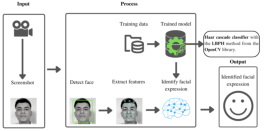
\includegraphics[frame,scale=0.5, width=\linewidth]{figs/Figure_2}
		\caption{Método para el reconocimiento de expresiones faciales utilizado en el sistema Torddis.\label{fig:FacialExpression}}
	\end{figure} 
	
	\subsubsection{Método para el Reconocimiento de Objetos}
	Este método consiste en los siguientes pasos:
	\begin{enumerate}
		\item Se toma una fotografía para capturar los objetos ubicados en el escritorio o el área donde el niño está trabajando.
		\item Se realiza el preprocesamiento de la imagen, seguido de la segmentación en partes correspondientes a los posibles objetos.
		\item Se lleva a cabo la extracción de características en la imagen segmentada.
		\item Finalmente, las características extraídas se comparan con un modelo computacional, que fue entrenado con un conjunto de imágenes que contienen los objetos que se espera reconocer.
	\end{enumerate}
	
	La visión por computadora permite la detección automática de la estructura y propiedades de un posible mundo dinámico en tres dimensiones, basándose en una o más imágenes bidimensionales del mundo \citep{Cruz2013}. La Figura \ref{fig:ObjectRecognition} ilustra el método de reconocimiento de objetos utilizado en la implementación del sistema Torddis.
	
	\begin{figure}[hbt!]
		\centering
		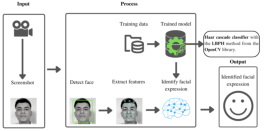
\includegraphics[frame,scale=0.5, width=\linewidth]{figs/Figure_3}
		\caption{Método para el reconocimiento de objetos utilizado en el sistema Torddis.\label{fig:ObjectRecognition}}
	\end{figure} 
	
	\subsubsection{Parámetros de Distracción}
	Para determinar los parámetros de distracción que afectan la concentración de los niños durante sus actividades escolares, se realizó una revisión bibliográfica. Además, se consideraron las opiniones de los usuarios y la aportación de un profesional de la educación. La Tabla \ref{tab:DistractionParameters} describe los parámetros de distracción acordados por consenso.
	
	\begin{table}[hbt!]
		\centering
		\caption{Parámetros de distracción en el área de estudio. \label{tab:DistractionParameters}}
		\begin{tabular}{p{0.46\textwidth}p{0.46\textwidth}}
			\hline
			\multicolumn{1}{l}{\rule{0pt}{2.5ex}\textbf{Distracción Interna}} & \multicolumn{1}{l}{\rule{0pt}{2.5ex}\textbf{Distracción Externa}} \\ \hline
			Expresión de emociones como ira, disgusto, miedo, felicidad, tristeza, sorpresa y neutral \citep{Asish2022Detecting,Vettivel2018System,Pabba2022AnIntelligent}. & Intervención de una persona desconocida o abandono del área de estudio \citep{Vettivel2018System}. \\ \hline
			Estado de somnolencia para determinar si el niño está despierto o dormido \citep{Pabba2022AnIntelligent}. & Objetos en el área de estudio que desvían la atención de las actividades que se están realizando \citep{Asish2022Detecting,Pabba2022AnIntelligent}. \\ \hline
		\end{tabular}
	\end{table}
	
	\subsubsection{Diagrama de Casos de Uso a Nivel General}
	En el diagrama general de casos de uso (ver Figura \ref{fig:UseCaseDiagram}), se muestran las funciones consideradas con base en las entrevistas iniciales con el usuario final y los educadores. El usuario tutor es la persona encargada de configurar los objetos permitidos, monitorizar a sus estudiantes, emitir alertas a los padres y persuadir a los niños monitoreados. Además, el usuario tutor puede visualizar los informes y los eventos históricos.
	
	\begin{figure}[hbt!]
		\centering
		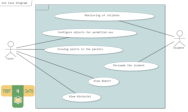
\includegraphics[frame,scale=0.5, width=\linewidth]{figs/Figure_4}
		\caption{Modelado de los requisitos del usuario a un nivel alto.\label{fig:UseCaseDiagram}}
	\end{figure} 
	
	\subsubsection{Análisis de Factibilidad}
	Este proyecto llevó a cabo un análisis de factibilidad en los tres aspectos considerados en la metodología TDDM4IoTS: factibilidad técnica, económica y operativa. La disponibilidad de los recursos de hardware y software necesarios para el desarrollo de Torddis fue crucial para garantizar el éxito de este proyecto. Además, la presencia de un equipo de desarrollo con las habilidades y conocimientos adecuados permitió completar Torddis con un presupuesto muy limitado y a tiempo.
	
	El equipo de proyecto logró reclutar a un usuario tutor con una necesidad inminente de un sistema como Torddis, permitiendo un análisis exhaustivo de necesidades. Además, se reclutó a un grupo de usuarios tutores para verificar los requisitos propuestos durante el desarrollo del proyecto y para evaluar la funcionalidad y usabilidad de Torddis. Se consideraron las capacidades de los usuarios tutores para garantizar que Torddis permaneciera operativo después de su implementación, sin la necesidad de personal adicional, excepto en casos de mantenimiento correctivo, donde personas con conocimientos sobre el desarrollo de Torddis tendrían que intervenir.
	
	\subsubsection{Análisis de Tecnologías}
	Se analizaron las tecnologías disponibles para el desarrollo de Torddis, incluyendo recursos de hardware, algoritmos y métodos de IA, y herramientas de software para monitorizar las distracciones de los estudiantes durante sus actividades escolares, según lo detallado en las distintas subsecciones de esta sección. Una revisión de los recursos existentes y su aplicación en entornos educativos ayudó a seleccionar las tecnologías más apropiadas para este proyecto.
	
	\subsubsection*{Recursos de Hardware}
	La Tabla \ref{table:hardware-components} describe los recursos de hardware IoT utilizados para construir Torddis. Se aplicaron los siguientes criterios para seleccionar los componentes de hardware:
	\begin{enumerate}
		\item \textbf{Precio:} El componente a adquirir debe ser económico.
		\item \textbf{Tiempo de entrega:} Dado que no existe un mercado directo para adquirirlo, se buscaron tiendas en línea (por ejemplo, www.mercadolibre.com.ec). La tienda debía ser confiable y el tiempo de entrega no debía superar las 48 horas.
		\item \textbf{Experiencia:} La experiencia del equipo de desarrollo en el uso del componente.
		\item \textbf{Documentación:} La disponibilidad de documentación en línea para el uso adecuado del componente seleccionado.
	\end{enumerate}
	
	\begin{table}[hbt!]
		\caption{Componentes de hardware.}
		\label{table:hardware-components}
		\centering
		\begin{tabular}{p{0.23\textwidth}p{0.15\textwidth}p{0.15\textwidth}p{0.35\textwidth}}
			\hline
			\multicolumn{1}{l}{\textbf{Funcionalidad}} & \multicolumn{1}{l}{\textbf{Seleccionado}} & \multicolumn{1}{l}{\textbf{Alternativas}} & \multicolumn{1}{l}{\textbf{Observación}} \\ \hline
			Conectividad con el servicio web y transmisión de video & Esp32cam & Cámara Ov7670 VGA & Este módulo tiene conectividad WiFi + Bluetooth y una cámara de video integrada \citep{CasasSanchez2022}. \\
			Transmisión de información & Esp8266 NodeMcu v3 & Arduino UNO, Módulo GSM & El módulo NodeMCU es una pequeña placa que proporciona conexión WiFi para la transmisión de datos al servicio web \citep{Barai2019}. \\
			Sonido de alarma & Zumbador pasivo & Zumbador activo & Comúnmente utilizado para generar alarmas sonoras en placas electrónicas \citep{Adebisi2023development}. \\
			Emisor de luz para alerta & LED de 5mm (cualquier color) & LED RGB & Diodo LED transparente brillante utilizado para configurar una alarma \citep{Upender2020}.  \\ \hline
		\end{tabular}
	\end{table}
	
	\subsubsection*{Tecnologías de Software}
	El desarrollo del sistema propuesto requirió el uso de diversas tecnologías, que abarcan lenguajes de programación y algoritmos de IA, para apoyar eficazmente el logro de los objetivos planteados. La Tabla \ref{table:software-technologies} presenta las tecnologías de software utilizadas en la construcción del sistema Torddis.
	
	\begin{table}[hbt!]
		\caption{Tecnologías de software utilizadas en la construcción del sistema Torddis.}
		\label{table:software-technologies}
		\centering
		\begin{tabular}{p{0.23\textwidth}p{0.15\textwidth}p{0.15\textwidth}p{0.35\textwidth}}
			\hline
			\multicolumn{1}{l}{\textbf{Funcionalidad}} & \multicolumn{1}{l}{\textbf{Alternativas }} & \multicolumn{1}{l}{\textbf{Seleccionado}} & \multicolumn{1}{l}{\textbf{Observación}} \\ \hline
			Aplicaciones móviles para Android & Kotlin & Java & Lenguaje utilizado en Android Studio con una gran comunidad en el campo del desarrollo de aplicaciones móviles \citep{Sharma2021Real-Time}. \\
			Aplicaciones de IA & Java, R & Python & Lenguaje de programación con bibliotecas de código abierto populares para el desarrollo de aplicaciones de IA \citep{Cai2005OnThePerformance}. \\
			Aplicaciones y servicios web & Flask & Django & Marco popular con capacidades de desarrollo rápido y previene errores de seguridad en el desarrollo de aplicaciones o servicios web \citep{Puneet2022ADjango}. \\
			Bases de datos & MySQL, Microsoft SQL Server & PostgreSQL & Base de datos robusta con mejor compatibilidad con el marco web Django \citep{Puneet2022ADjango}. \\ \hline
		\end{tabular}
	\end{table}
	
	\subsubsection*{Métodos de IA para monitorizar las Distracciones de los Niños}
	
	En esta etapa, se seleccionaron los métodos de IA más adecuados para desarrollar la propuesta de Torddis. Estos incluyen métodos para:
	\begin{itemize}
		\item Reconocimiento facial,
		\item Reconocimiento de expresiones faciales,
		\item Detección de sueño, y
		\item Reconocimiento de objetos.
	\end{itemize}
	
	\subsubsection*{Métodos para el Reconocimiento Facial}
	Los métodos de reconocimiento facial se centran en la detección de rostros, identificando patrones como ojos, labios, boca y nariz, entre otras partes. La Tabla \ref{tab:facial-recognition} enumera algunos métodos para detectar rostros y realizar reconocimiento facial.
	
	\begin{table}[h]
		\caption{Métodos para el reconocimiento facial.}
		\label{tab:facial-recognition}
		\centering
		\begin{tabular}{p{0.25\textwidth}p{0.23\textwidth}p{0.29\textwidth}p{0.23\textwidth}}
			\hline
			\multicolumn{1}{l}{\textbf{Método}} & \multicolumn{1}{l}{\textbf{Tecnología e Implementación}} & \multicolumn{1}{l}{\textbf{Uso}} & \multicolumn{1}{l}{\textbf{Precisión}} \\ \hline
			Clasificador Haar Cascade & \textit{(no especificado)} & Clasificación de género \citep{Priyanka2012Hybrid}. & \multicolumn{1}{r}{98.75\%} \\
			& OpenCV & Detección facial en entornos con poca luz \citep{Le2022Facial}. & \multicolumn{1}{r}{81.00\%} \\
			Amazon Rekognition & AWS & Autenticación mediante reconocimiento facial \citep{Girmay2021AI}. & \multicolumn{1}{r}{100\%} \\
			YOLO y MTCNN, FaceNet y SVC & Google Colab & Reconocimiento facial para control de asistencia \citep{Darapaneni2020Automatic}. & \multicolumn{1}{r}{99.00\%} \\
			Histograma de Patrones Binarios Locales (LBPH) & \textit{(no especificado)} & Detección facial a partir de imágenes capturadas \citep{Garcia2021Application}. & \multicolumn{1}{r}{91.72\%} \\ \hline
		\end{tabular}
	\end{table}
	La combinación de YOLO con MTCNN y FaceNet con SVC no es adecuada para el sistema propuesto debido a su complejidad y demanda computacional. Además, Amazon Rekognition fue descartado porque su procesamiento en la nube y personalización no son sencillos. Por lo tanto, el método seleccionado fue el clasificador Haar Cascade con el método LBPH de la biblioteca OpenCV, ya que su personalización es sencilla y el tiempo de resultado del reconocimiento es relativamente corto en comparación con otros.
	
	\subsubsection*{Métodos para el Reconocimiento de Expresiones Faciales}				
	El reconocimiento de expresiones faciales requiere una imagen de entrada para realizar la extracción de características, que luego se compara con un modelo computacional. La Tabla \ref{tab:facial-expression} enumera algunos métodos para la detección de expresiones faciales.
	
	Con base en la Tabla \ref{tab:facial-expression}, se eligió un algoritmo CNN para el desarrollo de Torddis debido a su precisión. Sin embargo, es importante asegurar un entrenamiento óptimo del modelo. Al decidir el algoritmo más adecuado para la implementación en un sistema, es necesario considerar que la precisión de algunos algoritmos depende del conjunto de datos utilizado. En el caso de MobileNetV2, se descartó debido a su menor precisión en el reconocimiento de expresiones faciales.
	
	\begin{table}[H]
		\caption{Métodos para el reconocimiento de expresiones faciales.}
		\label{tab:facial-expression}
		\centering
		\begin{tabular}{p{0.1\textwidth}p{0.12\textwidth}p{0.18\textwidth}p{0.30\textwidth}p{0.8\textwidth}}
			\hline
			\multicolumn{1}{l}{\textbf{Método}} & \multicolumn{1}{l}{\textbf{Conjunto de Datos}} & \multicolumn{1}{l}{\textbf{Tecnología e Implementación}} & \multicolumn{1}{l}{\textbf{Uso}} & \multicolumn{1}{l}{\textbf{Precisión}} \\ \hline
			Clasificador Haar Cascade & Personalizado & \textit{(no especificado)} & Reconoce siete expresiones: feliz, triste, enojado, asustado, disgustado, sorprendido y neutral \citep{Lalitha2021ADeep}. & \multicolumn{1}{r}{78.00\%} \\
			CNN & FERC 2013 & Python, Keras, Tensorflow y OpenCV & Reconocimiento de emociones humanas básicas (ira, miedo, neutral, feliz, triste, sorpresa, etc.). Implementado para la detección de emociones \citep{Kedari2021Face}. & \multicolumn{1}{r}{60.00\%} \\
			& \textit{(no especificado)} & CNN con 80 épocas & Genera y categoriza automáticamente preguntas, evalúa respuestas y rastrea el desempeño proporcionando citas motivacionales al detectar emociones del estudiante \citep{Silva2021AI}. & \multicolumn{1}{r}{99.00\%} \\ 
			MobileNetV2 & \textit{(no especificado)} & Python y TensorFlow & Evaluación en línea de la capacidad de los estudiantes para entrenar e implementar soluciones de aprendizaje profundo \citep{Ilic2021Automatic}. & \multicolumn{1}{r}{60.00\%} \\ \hline
		\end{tabular}
	\end{table}
	
	\subsubsection*{Métodos para el Reconocimiento de Objetos}				
	La visión por computadora permite la detección automática de la estructura y propiedades de un posible mundo dinámico tridimensional. Primero, se requiere una imagen de entrada que contenga uno o más objetos. Luego, se realiza el preprocesamiento de la imagen para extraer características de la imagen segmentada. La Tabla \ref{tab:object-recognition} describe una lista de algoritmos para el reconocimiento de objetos.
	
	Basado en la Tabla \ref{tab:object-recognition}, el algoritmo seleccionado fue Sequential de la biblioteca TensorFlow en combinación con Keras debido a su precisión, rendimiento óptimo, facilidad de entrenamiento y uso generalizado para el reconocimiento de objetos en tiempo real. MobileNetV2 combinado con SSD se descartó debido a su menor precisión en el reconocimiento de objetos en comparación con otros. Además, YOLO fue descartado debido al alto consumo de GPU (Unidad de Procesamiento Gráfico) requerido para su correcto funcionamiento.
	
	\begin{table}[ht!]
		\caption{Algoritmos para el reconocimiento de objetos.}
		\label{tab:object-recognition}
		\centering
		\begin{tabular}{p{0.1\textwidth}p{0.32\textwidth}p{0.39\textwidth}p{0.8\textwidth}}
			\hline
			\multicolumn{1}{l}{\textbf{Algoritmo}} & \multicolumn{1}{l}{\textbf{Tecnología e Implementación}} & \multicolumn{1}{l}{\textbf{Uso}} & \multicolumn{1}{l}{\textbf{Precisión}} \\ \hline
			YOLO & YOLOv4 & Reconocimiento de objetos \citep{Liu2021Objetcs}. & \multicolumn{1}{r}{73.01\%} \\
			Sequential TensorFlow & Keras & Clasificación y detección de imágenes aéreas \citep{Sudharshan2018Object}. & \multicolumn{1}{r}{96.00\%} \\ \hline
		\end{tabular}
	\end{table}
	
	\subsubsection*{Métodos para la Detección de Sueño}
	Los métodos para la detección de sueño requieren una imagen que contenga un rostro como entrada. Estos métodos realizan el preprocesamiento de la imagen para extraer los puntos característicos de los ojos y luego analizan si la persona tiene los ojos cerrados. La Tabla \ref{tab:sleep-detection-methods} enumera los métodos para la detección de sueño.
	
	\begin{table}[h]
		\centering
		\caption{Métodos para la detección de sueño.}
		\label{tab:sleep-detection-methods}
		\begin{tabular}{p{0.35\textwidth}p{0.43\textwidth}p{0.10\textwidth}}
			\hline
			\multicolumn{1}{c}{\rule{0pt}{2.5ex}\textbf{Algoritmo}} & \multicolumn{1}{c}{\rule{0pt}{2.5ex}\textbf{\parbox{3cm}{Uso}}} & \multicolumn{1}{c}{\rule{0pt}{2.5ex}\textbf{Precisión}} \\ \hline
			MediaPipe Face Mesh & Detección de puntos característicos faciales con 468 puntos 3D \citep{Shanmugam2022Comparative}. & \multicolumn{1}{r}{99.87\%} \\ 
			SVM & Seguimiento de ojos \citep{Altameem2021Early}. & \multicolumn{1}{r}{83.25\%} \\
			CNN & Entrenado con 4 gestos, como ojos abiertos, ojos cerrados, bostezando y no bostezando \citep{Diagram2023Software}. & \multicolumn{1}{r}{80.00\%} \\ \hline
		\end{tabular}
	\end{table}
		
	\subsection{Generación del Software}
	En esta etapa, se escribió el código del software basado en los modelos y pruebas generados por TDDT4IoTS. Gran parte del software fue generado automáticamente y el resto fue completado por los desarrolladores. Se utilizó Python para implementar los servicios web, Java para desarrollar la aplicación móvil y C++ junto con el IDE de Arduino para configurar los componentes del dispositivo Torddis. Una vez que el software se generó automáticamente y de forma manual, se verificó con las pruebas correspondientes. En resumen, en esta etapa se obtuvieron componentes de software funcionales y probados para cada entregable.
	
	\subsection{Refinamiento del Modelo}
	Esta etapa es importante cuando los requisitos no están claros al inicio del desarrollo y se vuelven más específicos a medida que avanza el ciclo de vida del proyecto. Durante esta fase de refinamiento, se obtuvieron versiones mejoradas de los modelos del sistema para cada entregable, proporcionando una solución más integral. En el caso particular de Torddis, los modelos UML iniciales se actualizaron mediante la especificación de los casos de uso correspondientes, permitiendo que TDDT4IoTS generara modelos mejorados. Además, los modelos computacionales de IA se refinaron para monitorizar los parámetros de distracción de los niños, ajustando configuraciones como el número de capas ocultas y las épocas de entrenamiento del modelo.
	
	\subsection{Refinamiento del Software}
	Esta etapa de refinamiento resultó en un software mejorado, con código más limpio y de mayor calidad en comparación con el entregable de la etapa anterior. Las herramientas utilizadas para la tarea de refinamiento de software, con la excepción de TDDT4IoTS, fueron equivalentes a las utilizadas en la etapa de generación de software. Los cambios realizados en el software consistieron principalmente en mejoras relacionadas con el uso de la memoria (reducción de variables temporales o auxiliares), el nombrado de atributos, métodos y clases (archivos del proyecto), y en la inclusión de comentarios en las partes más importantes del código.
	
	\subsection{Despliegue de Hardware y Software}
	La aplicación móvil se desplegó en un smartphone con Android versión 13, Xiaomi Note 10 Pro, para realizar pruebas de evaluación llevadas a cabo por el interesado (uno de los padres de los niños en edad escolar). Esta aplicación consume servicios web alojados en un servidor web.
	
	El dispositivo Torddis se desplegó en un entorno real-ideal, donde cualquier niño puede realizar tareas escolares.
	
	La Figura \ref{fig:Torddis} muestra capturas de pantalla tanto de la aplicación móvil como del dispositivo Torddis, destacando su diseño intuitivo y las funciones clave para la monitorización en tiempo real de las distracciones de los estudiantes. Además, se muestra el dispositivo IoT, integrando tecnologías de reconocimiento facial y detección de objetos, proporcionando un apoyo integral para mejorar la concentración académica en el hogar. La Figura \ref{fig:Torddis}a muestra las diferentes opciones disponibles para el tutor, mientras que la Figura \ref{fig:Torddis}b muestra la lista de estudiantes bajo la supervisión de un tutor. Por otro lado, la Figura \ref{fig:Torddis}c muestra el dispositivo Torddis en sí.
	
	\begin{figure}[hbt!]
		\centering
		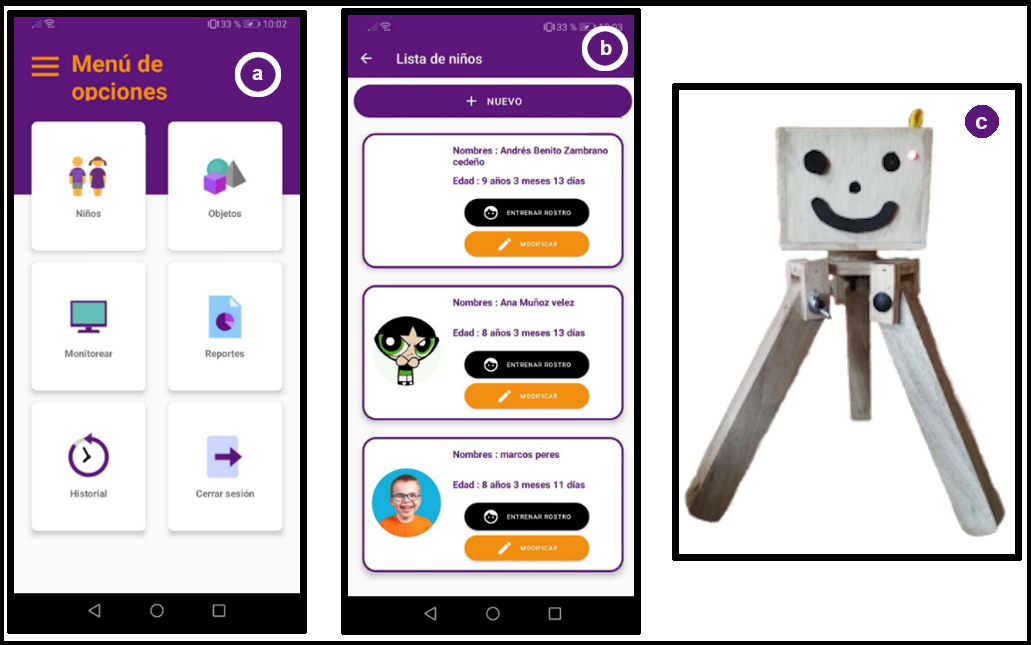
\includegraphics[width=\linewidth]{figs/Figure_9}
		\caption{Capturas de pantalla de la aplicación móvil y dispositivo del sistema Torddis.\label{fig:Torddis}} 
	\end{figure}
	
	\subsection{Evaluación del Entregable}
	La Figura \ref{fig:ConfigEvaluation} muestra la configuración del entorno utilizado para evaluar el sistema Torddis. En dicha figura, se puede observar que el niño está sentado en un escritorio realizando actividades académicas mientras el sistema Torddis monitorea su concentración y distracciones. El dispositivo Torddis se coloca a una distancia de entre 50 y 70 cm del niño, lo cual es crucial para el correcto funcionamiento de las tecnologías de reconocimiento facial y de objetos. Cabe mencionar que, para el niño, este dispositivo está destinado a ser percibido como un adorno decorativo en su escritorio.
	
	\begin{figure}[hbt!]
		\centering
		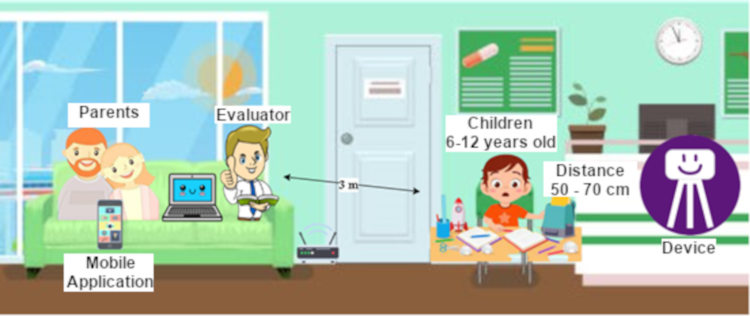
\includegraphics[width=\linewidth]{figs/Figure_10}
		\caption{Configuración del entorno para la evaluación del sistema Torddis. \label{fig:ConfigEvaluation}} 
	\end{figure}
	
	Un evaluador, uno de los autores de este trabajo, se encuentra posicionado a unos 3 metros del niño, supervisando el funcionamiento del sistema a través de una laptop. Uno o ambos padres están presentes, utilizando la aplicación móvil integrada con el dispositivo para monitorizar la concentración del niño en tiempo real, así como consultar la información resultante del procesamiento de los datos recopilados y analizados.
	
	Esta configuración permitió una evaluación integral del sistema Torddis, asegurando que todos los involucrados (niños, padres y evaluadores) pudieran interactuar con la tecnología y proporcionar información valiosa sobre su efectividad en la monitorización y mejora de la concentración académica en un entorno controlado.
	
	Las Tablas \ref{tab:create-tutor-account-test-case}, \ref{tab:login-test-case}, \ref{tab:face-training-test-case}, \ref{tab:device-registration-test-case}, y \ref{tab:configure-object-usage-test-case} muestran algunos de los casos de prueba funcionales ejecutados por el usuario. Estos son los casos de prueba con los cuales los interesados verifican que Torddis cumple con los requisitos especificados.
	
	\begin{table}[hbt!]
		\centering
		\caption{Caso de prueba para la creación de la cuenta de tutor.}
		\label{tab:create-tutor-account-test-case}
		\begin{tabularx}{\textwidth}{l X}
			\toprule
			\textbf{Código del Caso de Prueba:} & PU-1 \\
			\textbf{Nombre del Caso de Prueba:} & Creación de Cuenta de Tutor \\
			\textbf{Resultado Esperado:} & Crear con éxito una cuenta de tutor \\
			\midrule
			\multicolumn{2}{c}{\textbf{Procedimiento del Caso de Prueba}} \\
			\midrule
			\multicolumn{1}{c}{\textbf{No.}} & \textbf{Descripción del Paso} \\
			\midrule
			\multicolumn{1}{c}{1} & Abrir la aplicación móvil. \\
			\multicolumn{1}{c}{2} & Seleccionar la opción "Registrarse". \\
			\multicolumn{1}{c}{3} & Ingresar los datos de registro.
			\begin{itemize}
				\item Nombre: Carlos Iván
				\item Apellidos: Almeida Dueñas
				\item Correo electrónico: carlos.almeida2017@utec.edu.ec
				\item Fecha de nacimiento: 10/01/2000
				\item Nombre de usuario: calmeidad
				\item Contraseña: XXXXXX
			\end{itemize}\\
			\multicolumn{1}{c}{4} & Seleccionar la opción "Crear Cuenta". \\
			\bottomrule
		\end{tabularx}
	\end{table}
	
	\begin{table}[hbt!]
		\centering
		\caption{Caso de prueba para iniciar sesión.}
		\label{tab:login-test-case}
		\begin{tabularx}{\textwidth}{l X}
			\toprule
			\textbf{Código del Caso de Prueba:} & PU-2 \\
			\textbf{Nombre del Caso de Prueba:} & Inicio de Sesión \\
			\textbf{Resultado Esperado:} & Iniciar sesión exitosamente con una cuenta de tutor \\ \midrule
			\multicolumn{2}{c}{\textbf{Procedimiento del Caso de Prueba}} \\ \midrule
			\multicolumn{1}{c}{\textbf{No.}} & \textbf{Descripción del Paso} \\ \midrule
			\multicolumn{1}{c}{1} & Ingresar las credenciales de inicio de sesión.
			\begin{itemize}
				\item Nombre de usuario: calmeidad
				\item Contraseña: XXXXXX
			\end{itemize} \\
			\multicolumn{1}{c}{2} & Seleccionar la opción "Iniciar Sesión". \\
			\multicolumn{1}{c}{3} & La aplicación móvil muestra la pantalla del menú del usuario tutor. \\
			\bottomrule
		\end{tabularx}
	\end{table}
	
	\begin{table}[hbt!]
		\centering
		\caption{Caso de prueba para el entrenamiento facial.}
		\label{tab:face-training-test-case}
		\begin{tabularx}{\textwidth}{l X}
			\toprule
			\textbf{Código del Caso de Prueba:} & PU-3 \\
			\textbf{Nombre del Caso de Prueba:} & Entrenamiento Facial \\
			\textbf{Resultado Esperado:} & Realizar con éxito el entrenamiento facial para un estudiante\\
			\midrule
			\multicolumn{2}{c}{\textbf{Procedimiento del Caso de Prueba}} \\
			\midrule
			\multicolumn{1}{c}{\textbf{No.}} & \textbf{Descripción del Paso} \\
			\midrule
			\multicolumn{1}{c}{1} & Ingresar al módulo "Niño" de la aplicación. \\
			\multicolumn{1}{c}{2} & Seleccionar la opción "Entrenar" para un niño. \\
			\multicolumn{1}{c}{3} & Registrar un dispositivo (ver caso de prueba Tabla \ref{tab:device-registration-test-case}). \\
			\multicolumn{1}{c}{4} & Seleccionar la opción "Entrenar". \\
			\multicolumn{1}{c}{5} & Colocar el rostro del niño frente a la cámara del dispositivo y esperar a que se complete el proceso de entrenamiento facial. \\
			\bottomrule
		\end{tabularx}
	\end{table}
	
	\begin{table}[hbt!]
		\centering
		\caption{Caso de prueba para el registro del dispositivo.}
		\label{tab:device-registration-test-case}
		\begin{tabularx}{\textwidth}{l X}
			\toprule
			\textbf{Código del Caso de Prueba:} & PU-4 \\
			\textbf{Nombre del Caso de Prueba:} & Registro del Dispositivo \\
			\textbf{Resultado Esperado:} & Registrar con éxito el dispositivo en la aplicación móvil \\
			\midrule
			\multicolumn{2}{c}{\textbf{Procedimiento del Caso de Prueba}} \\
			\midrule
			\multicolumn{1}{c}{\textbf{No.}} & \textbf{Descripción del Paso} \\
			\midrule
			\multicolumn{1}{c}{1} & Seleccionar la opción "Registrar Dispositivo". \\
			\multicolumn{1}{c}{2} & Ingresar la dirección IP del dispositivo. \\
			\multicolumn{1}{c}{3} & Seleccionar la opción "Guardar". \\
			\bottomrule
		\end{tabularx}
	\end{table}
	
	\begin{table}[hbt!]
		\centering
		\caption{Caso de prueba para configurar el uso de objetos.}
		\label{tab:configure-object-usage-test-case}
		\begin{tabularx}{\textwidth}{l X}
			\toprule
			\textbf{Código del Caso de Prueba:} & PU-5 \\
			\textbf{Nombre del Caso de Prueba:} & Configuración del Uso de Objetos \\
			\textbf{Resultado Esperado:} & Configurar con éxito el uso de objetos \\
			\midrule
			\multicolumn{2}{c}{\textbf{Procedimiento del Caso de Prueba}} \\
			\midrule
			\multicolumn{1}{c}{\textbf{No.}} & \textbf{Descripción del Paso} \\
			\midrule
			\multicolumn{1}{c}{1} & Ingresar al módulo "Objetos" de la aplicación. \\
			\multicolumn{1}{c}{2} & Buscar el objeto que se desea activar/desactivar. \\
			\multicolumn{1}{c}{3} & Seleccionar el control de interruptor de un objeto para activarlo/desactivarlo. \\
			\bottomrule
		\end{tabularx}
	\end{table}
	
	\subsection{Mantenimiento}
	Esta fase no fue ejecutada debido al corto tiempo de desarrollo para cada entregable, y por lo tanto, para el proyecto. Sin embargo, el sistema debe ser mantenido para funcionar correctamente. La Tabla \ref{tab:maintenance-tasks} describe algunas tareas de mantenimiento tentativas que deben considerarse de manera trimestral y semestral, aunque su frecuencia puede variar dependiendo del contexto.
	
	\begin{table}[hbt!]
		\centering
		\caption{Definición de tareas de mantenimiento.}
		\label{tab:maintenance-tasks}
		\begin{tabularx}{\textwidth}{cXcc}
			\toprule
			\textbf{No.} & \textbf{Tareas de Mantenimiento} & \textbf{Trimestral} & \textbf{Semestral} \\
			\midrule
			1 & Limpieza interna del dispositivo. & * & \\
			2 & Verificar si los componentes del dispositivo tienen alguna imperfección o daño. & & * \\
			3 & Comprobar conexiones de cables, estado de los cables, conectores, etc. & & * \\
			4 & Probar el funcionamiento del zumbador y los LED. & * & \\
			5 & Probar el sistema informático (servidor de aplicaciones web, servicios web, aplicación móvil, dispositivo IoT). & & * \\
			\bottomrule
		\end{tabularx}
	\end{table}
	
	```latex
	\section{Resultados y Discusión}
	\label{seccion:Cinco}
	En esta sección se presentan los hallazgos obtenidos a través de diversas evaluaciones realizadas al prototipo del sistema Torddis. Estas evaluaciones incluyen pruebas funcionales, cuestionarios de usabilidad y análisis de datos demográficos y de monitorización, con el objetivo de determinar la efectividad y aceptación del sistema desde una perspectiva tanto técnica como de experiencia del usuario. Los resultados de estas evaluaciones se detallan a continuación, proporcionando una visión integral del rendimiento y utilidad del sistema Torddis en su contexto de aplicación.
	
	\subsection{Análisis de Reconocimiento}
	Esta subsección presenta los resultados de 14 pruebas realizadas utilizando el sistema Torddis, en las cuales se evaluaron cuatro tareas diferentes de reconocimiento: personas, expresiones faciales, presencia de sueño y objetos distractores. Cada prueba midió el tiempo en segundos que tomó reconocer el elemento correspondiente y registró si el reconocimiento fue exitoso o no. La Tabla \ref{tab:combined-recognition} muestra los datos recopilados para este análisis.
	
	\begin{table}[hbt!]
		\centering
		\caption{Resultados agregados de reconocimiento.}
		\label{tab:combined-recognition}
		\begin{tabularx}{\textwidth}{c >{\centering\arraybackslash}X c >{\centering\arraybackslash}X c >{\centering\arraybackslash}X c >{\centering\arraybackslash}X c}
			\toprule
			\textbf{No.} & \multicolumn{2}{c}{\textbf{Personas}} & \multicolumn{2}{c}{\textbf{Expresiones Faciales}} & \multicolumn{2}{c}{\textbf{Presencia de Sueño}} & \multicolumn{2}{c}{\textbf{Objetos Distractores}}\\
			\cline{2-9}
			& \textbf{Latencia} & \textbf{Logrado?} & \textbf{Latencia} & \textbf{Logrado?} & \textbf{Latencia} & \textbf{Logrado?} & \textbf{Latencia} & \textbf{Logrado?} \\
			\midrule
			1 & 0.57 & Sí & 1.50 & Sí & 5.10 & Sí & 0.00 & \textbf{No} \\
			2 & 0.60 & Sí & 1.20 & Sí & 3.50 & Sí & 1.68 & Sí \\
			3 & 0.00 & \textbf{No} & 0.70 & Sí & 0.00 & \textbf{No} & 0.00 & No \\
			4 & 0.78 & Sí & 1.30 & Sí & 3.68 & Sí & 1.79 & Sí \\
			5 & 1.02 & Sí & 0.78 & Sí & 2.24 & Sí & 0.00 & \textbf{No} \\
			6 & 0.88 & Sí & 1.01 & \textbf{No} & 2.63 & Sí & 1.98 & Sí \\
			7 & 0.53 & Sí & 1.23 & Sí & 0.00 & \textbf{No} & 1.73 & Sí \\
			8 & 1.20 & Sí & 0.97 & Sí & 2.03 & Sí & 2.05 & Sí \\
			9 & 0.76 & Sí & 1.05 & Sí & 4.09 & Sí & 1.77 & Sí \\
			10 & 1.20 & Sí & 0.70 & Sí & 3.36 & Sí & 1.91 & Sí \\
			11 & 0.69 & Sí & 1.99 & Sí & 4.69 & Sí & 4.27 & Sí \\
			12 & 0.82 & Sí & 1.83 & Sí & 3.29 & Sí & 2.69 & Sí \\
			13 & 0.93 & Sí & 1.68 & Sí & 3.14 & Sí & 2.81 & Sí \\
			14 & 0.58 & Sí & 1.76 & Sí & 3.45 & Sí & 2.94 & Sí \\
			\bottomrule
		\end{tabularx}
	\end{table}
	
	\subsubsection{Resultados}
	\begin{itemize}
		\item \textbf{Tiempo total de reconocimiento en segundos para todas las pruebas}: 
		\begin{itemize}
			\item Personas: 10.56 segundos
			\item Expresiones Faciales: 17.70 segundos
			\item Sueño: 41.20 segundos
			\item Objetos Distractores: 25.62 segundos
		\end{itemize}
		\item \textbf{Número de reconocimientos exitosos}:
		\begin{itemize}
			\item Personas: 13
			\item Expresiones Faciales: 13
			\item Sueño: 12
			\item Objetos Distractores: 11
		\end{itemize}
		\item \textbf{Número de fallos en el reconocimiento}:
		\begin{itemize}
			\item Personas: 1
			\item Expresiones Faciales: 1
			\item Sueño: 2
			\item Objetos Distractores: 3
		\end{itemize}
	\end{itemize}
	
	\subsubsection{Tiempo Promedio de Reconocimiento}
	El tiempo promedio para los reconocimientos exitosos se calculó para cada tarea de reconocimiento:
	
	\begin{itemize}
		\item \textbf{Personas}: \(\frac{10.56 \text{ segundos}}{13} \approx 0.81 \text{ segundos}\)
		\item \textbf{Expresiones Faciales}: \(\frac{17.70 \text{ segundos}}{13} \approx 1.36 \text{ segundos}\)
		\item \textbf{Sueño}: \(\frac{41.20 \text{ segundos}}{12} \approx 3.43 \text{ segundos}\)
		\item \textbf{Objetos Distractores}: \(\frac{25.62 \text{ segundos}}{11} \approx 2.33 \text{ segundos}\)
	\end{itemize}
	
	\subsubsection{Tasa de Reconocimiento}
	La tasa de reconocimiento se determinó para cada tarea como el porcentaje de reconocimientos exitosos sobre el total de pruebas:
	
	\begin{itemize}
		\item \textbf{Personas}: \(92.86\%\)
		\item \textbf{Expresiones Faciales}: \(92.86\%\)
		\item \textbf{Sueño}: \(85.71\%\)
		\item \textbf{Objetos Distractores}: \(78.57\%\)
	\end{itemize}
	
	\subsubsection{Tiempos Mínimos y Máximos de Reconocimiento}
	Tiempos mínimos y máximos de reconocimiento observados en las pruebas para cada tarea:
	
	\begin{itemize}
		\item \textbf{Personas}:
		\begin{itemize}
			\item Tiempo mínimo: 0.00 segundos (Prueba 3)
			\item Tiempo máximo: 1.20 segundos (Pruebas 8 y 10)
		\end{itemize}
		\item \textbf{Expresiones Faciales}:
		\begin{itemize}
			\item Tiempo mínimo: 0.70 segundos (Pruebas 3 y 10)
			\item Tiempo máximo: 1.99 segundos (Prueba 11)
		\end{itemize}
		\item \textbf{Sueño}:
		\begin{itemize}
			\item Tiempo mínimo: 0.00 segundos (Pruebas 3 y 7)
			\item Tiempo máximo: 5.10 segundos (Prueba 1)
		\end{itemize}
		\item \textbf{Objetos Distractores}:
		\begin{itemize}
			\item Tiempo mínimo: 0.00 segundos (Pruebas 1, 3 y 5)
			\item Tiempo máximo: 4.27 segundos (Prueba 11)
		\end{itemize}
	\end{itemize}
	
	\subsubsection{Distribución de los Tiempos de Reconocimiento}
	Los tiempos de reconocimiento para cada tarea varían, lo que indica una variabilidad en la respuesta del sistema. La mayoría de los tiempos de reconocimiento están dentro de un rango razonable, lo que sugiere una respuesta rápida y efectiva del sistema en la mayoría de los casos.
	
	\subsection{Evaluación de Usabilidad del Sistema Prototipo Desarrollado}
	La evaluación de la usabilidad del sistema Torddis se llevó a cabo para recopilar información sobre la experiencia general del usuario, centrándose específicamente en la facilidad de uso, la interfaz del sistema y la efectividad de las funciones proporcionadas. Esta evaluación integral tuvo como objetivo identificar fortalezas y áreas de mejora, asegurando que el sistema cumpla eficazmente con las necesidades de los usuarios. Las siguientes subsecciones detallan los datos demográficos de los participantes, sus experiencias, las tareas específicas realizadas durante la evaluación y los resultados del cuestionario SUS y de las preguntas abiertas (ver Apéndice \ref{Appendix:SUSQuestionarie}).
	
	\subsubsection{Datos Demográficos}
	Al inicio de la evaluación de usabilidad, se proporcionó un cuestionario demográfico para recopilar información sobre los tutores que participaron en la evaluación de usabilidad del sistema Torddis (ver Apéndice \ref{Appendix:DemographicSurvey}). El cuestionario demográfico arrojó los siguientes resultados:
	
	\begin{itemize}
		\item Se evaluaron un total de 12 familias: 8 madres y 4 padres, todos pertenecientes a la zona geográfica de Quevedo, Ecuador.
		\item La edad promedio de los participantes es de 39 años, con un rango de edad entre 18 y 65 años.
		\item El 58\% de los tutores solo completaron la educación primaria, mientras que el 42\% estudiaron hasta la educación secundaria.
	\end{itemize}
	
	\subsubsection{Acerca dla monitorización}
	Una de las preguntas preliminares en la evaluación de usabilidad fue sobre la facilidad con la que pueden monitorizar a sus hijos de primaria mientras realizan sus tareas escolares (ver Figura \ref{fig:previous-questions}). La mayoría de los tutores respondieron que el proceso de monitorización de la distracción de los niños es una tarea compleja. La Figura \ref{fig:monitoring-process} muestra los resultados detallados. Otra pregunta preliminar fue sobre la frecuencia con la que necesitaban monitorizar a sus hijos mientras realizaban actividades escolares. La mayoría de los tutores indicaron que debían hacerlo constantemente. Para respuestas más detalladas, véase la Figura \ref{fig:monitoring-frequency}. Finalmente, los tutores indicaron que, entre las estrategias que utilizan para mantener a sus estudiantes concentrados en sus actividades escolares, están las llamadas de atención (regaños), los consejos motivacionales y las recompensas, tales como dulces, juguetes, paseos al parque, comidas favoritas, y así sucesivamente (ver Figura \ref{fig:concentration-strategies}).
	
	\begin{figure}[hbt!]
		\centering
		\begin{minipage}{0.45\textwidth}
			\centering
			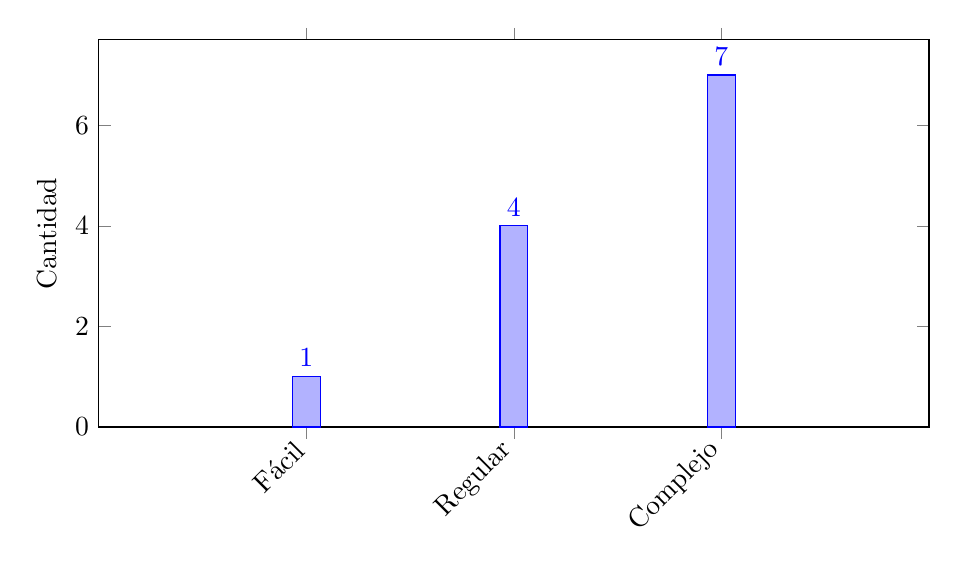
\begin{tikzpicture}
				\begin{axis}[
					ybar,
					width=\textwidth,
					height=6.5cm,
					symbolic x coords={Fácil, Regular, Complejo},
					xtick=data,
					ylabel={Cantidad},
					ymin=0,
					nodes near coords,
					enlarge x limits=0.5,
					x tick label style={rotate=45, anchor=east}
					]
					\addplot coordinates {(Fácil, 1) (Regular, 4) (Complejo, 7)};
				\end{axis}
			\end{tikzpicture}
			\subcaption{Facilidad del proceso de monitorización.}
			\label{fig:monitoring-process}
		\end{minipage}
		\vspace{5mm}
		\begin{minipage}{0.45\textwidth}
			\centering
			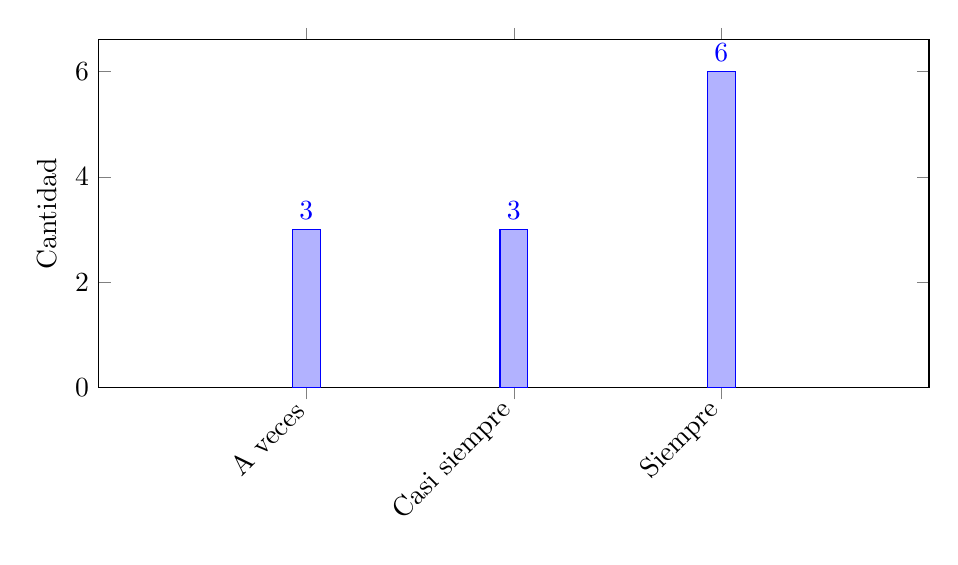
\begin{tikzpicture}
				\begin{axis}[
					ybar,
					width=\textwidth,
					height=6cm,
					symbolic x coords={A veces, Casi siempre, Siempre},
					xtick=data,
					ylabel={Cantidad},
					ymin=0,
					nodes near coords,
					enlarge x limits=0.5,
					x tick label style={rotate=45, anchor=east}
					]
					\addplot coordinates {(A veces, 3) (Casi siempre, 3) (Siempre, 6)};
				\end{axis}
			\end{tikzpicture}
			\subcaption{Frecuencia de monitorización.}
			\label{fig:monitoring-frequency}
		\end{minipage}
		\begin{minipage}{0.45\textwidth}
			\centering
			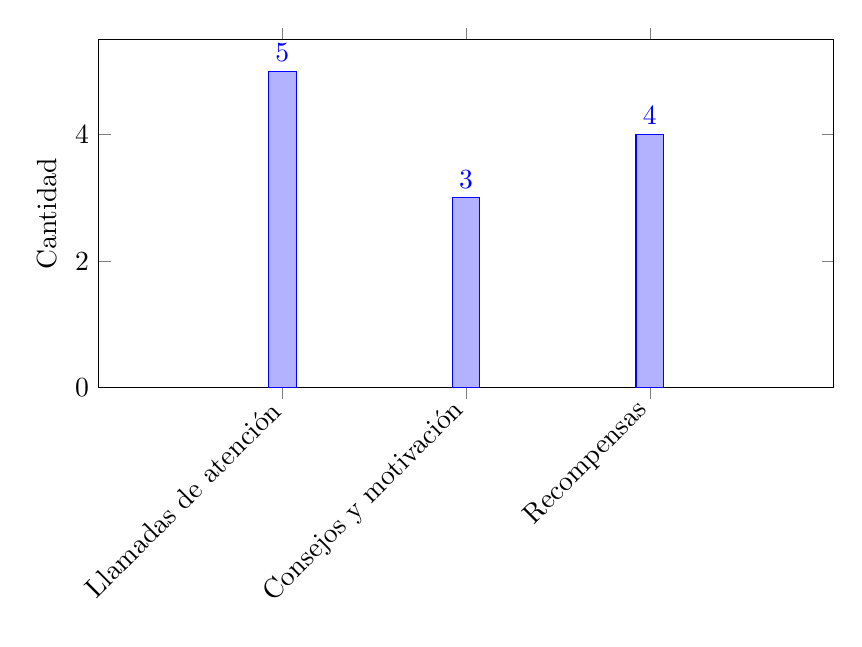
\begin{tikzpicture}
				\begin{axis}[
					ybar,
					height=6cm,
					width=0.9\textwidth,
					symbolic x coords={Llamadas de atención, Consejos y motivación, Recompensas},
					xtick=data,
					ylabel={Cantidad},
					ymin=0,
					nodes near coords,
					enlarge x limits=0.5,
					x tick label style={rotate=45, anchor=east}
					]
					\addplot coordinates {(Llamadas de atención, 5) (Consejos y motivación, 3) (Recompensas, 4)};
				\end{axis}
			\end{tikzpicture}
			\subcaption{Estrategias para lograr la concentración.}
			\label{fig:concentration-strategies}
		\end{minipage}
		\caption{Resultados de preguntas realizadas a los padres sobre el proceso de monitorización de sus hijos de primaria mientras hacen sus tareas.}
		\label{fig:previous-questions}
	\end{figure}
	
	```latex
	\subsubsection{Tareas para los Usuarios Participantes}
	Las tareas que los tutores realizaron durante la evaluación fueron las siguientes:
	
	\begin{enumerate}
		\item Conectar el dispositivo Torddis a la fuente de alimentación y colocarlo en el escritorio donde el niño se sentará para realizar una tarea.
		\item Crear una cuenta de usuario tutor en la aplicación móvil.
		\item Iniciar sesión en la aplicación móvil.
		\item Registrar al niño que será monitoreado.
		\item Registrar el dispositivo Torddis en la aplicación móvil utilizando la dirección IP proporcionada en una etiqueta adherida al dispositivo.
		\item Realizar el entrenamiento facial para el niño registrado.
		\item Activar y/o desactivar los objetos que se monitorizarán en la sección correspondiente de la aplicación móvil.
		\item Asignar una tarea al niño mientras es monitoreado por el dispositivo Torddis: colorear un mandala.
		\item Activar el reconocimiento de cada parámetro de distracción en la sección de monitorización de la aplicación móvil.
		\item Dejar al niño solo, sin la presencia de un adulto, durante 6 minutos.
		\item Activar y/o desactivar la transmisión de video desde el dispositivo Torddis.
		\item Navegar por el historial de los parámetros de distracción monitoreados en el niño.
		\item Visualizar un informe con gráficos que representan los parámetros de distracción detectados para el niño monitoreado.
	\end{enumerate}
	
	\subsubsection{Resultados del Cuestionario System Usability Scale}
	Los resultados analizados en esta sección corresponden a las respuestas del cuestionario SUS (ver Apéndice \ref{Appendix:LikertScale}) proporcionado a los 12 tutores. Después de tabular los datos obtenidos, la Figura \ref{fig:sus-questionnaire} muestra que la media de los datos recopilados es 81.46\% con una desviación estándar de 11.65. Según los adjetivos (Peor imaginable, Pobre, OK, Bueno, Excelente, Mejor imaginable) propuestos por Bangor et al. \cite{Bangor2008AnEmpirical} para evaluar cualitativamente la usabilidad de un sistema basado en la media alcanzada, es evidente que Torddis tiene un nivel de usabilidad "Bueno" según los tutores evaluados.
	
	\begin{figure}[hbt!]
		\centering
		\begin{tikzpicture}
			\begin{axis}[
				scatter/classes={
					a={mark=*,blue}
				},
				width=12cm,
				height=8cm,
				xlabel={Participante},
				ylabel={Evaluación},
				ymin=40, ymax=100,
				xmin=0, xmax=13,
				xtick={1,2,3,4,5,6,7,8,9,10,11,12},
				xticklabels={1,2,3,4,5,6,7,8,9,10,11,12},
				ytick={40,60,80,100},
				nodes near coords,
				every node near coord/.append style={font=\footnotesize, /pgf/number format/fixed},
				legend style={at={(0.5,-0.15)}, anchor=north, legend columns=-1},
				enlarge x limits=0.05,
				]
				\addplot[
				scatter,
				only marks,
				scatter src=explicit symbolic,
				visualization depends on=\thisrow{Evaluation} \as \label
				] table[meta=class,x=Participant,y=Evaluation] {
					Participant Evaluation class
					1 90.00 90.00
					2 95.00 95.00
					3 72.50 72.50
					4 60.00 60.00
					5 85.00 85.00
					6 67.50 67.50
					7 92.50 92.50
					8 67.50 67.50
					9 82.50 82.50
					10 85.00 85.00
					11 92.50 92.50
					12 87.50 87.50
				};
				
				% Línea de promedio
				\addplot [
				color=orange,
				thick,
				mark=none
				] coordinates {(0,\average) (13,\average)};
				
				% Línea de desviación estándar superior
				\addplot [
				color=orange,
				thick,
				dashed,
				mark=none
				] coordinates {(0,\upperlimit) (13,\upperlimit)};
				
				% Línea de desviación estándar inferior
				\addplot [
				color=orange,
				thick,
				dashed,
				mark=none
				] coordinates {(0,\lowerlimit) (13,\lowerlimit)};
				
				\legend{Participante, Promedio SUS, Desv. Estándar}
			\end{axis}
		\end{tikzpicture}
		\caption{Datos del cuestionario SUS por tutor con evaluación promedio y desviación estándar.}
		\label{fig:sus-questionnaire}
	\end{figure}
	
	\subsubsection{Resultados del Cuestionario de Preguntas Abiertas}
	Al final del cuestionario SUS, los tutores respondieron 8 preguntas abiertas (ver Apéndice \ref{Appendix:OpenQuestions}) para proporcionar sus opiniones personales.
	
	La primera pregunta fue "¿Cuál es su opinión general sobre el sistema?", a la que algunos tutores respondieron que apoya la concentración de los estudiantes, y otros dijeron que tiene un diseño agradable. Los resultados se muestran en la Figura \ref{fig:AboutTorddis}. La segunda pregunta abierta que respondieron los tutores fue "¿Le gustaron los sonidos y/o luces que utiliza Torddis?". La mayoría de los tutores presentaron una opinión favorable a esta pregunta, ya que creen que las alertas luminosas ayudan a mantener al estudiante despierto y están satisfechos con las alarmas sonoras (ver Figura \ref{fig:SoundAndLigth}).
	
	\begin{figure}[hbt!]
		\centering
		\begin{minipage}{0.45\textwidth}
			\centering
			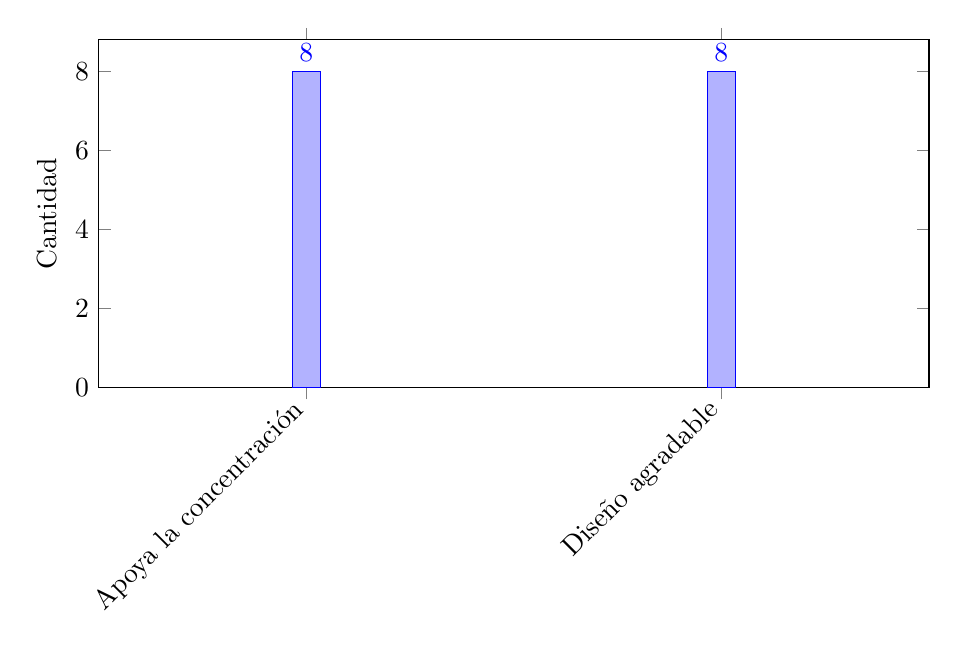
\begin{tikzpicture}
				\begin{axis}[
					ybar,
					width=\textwidth,
					height=6cm,
					symbolic x coords={Apoya la concentración, Diseño agradable},
					xtick=data,
					ylabel={Cantidad},
					ymin=0,
					nodes near coords,
					enlarge x limits=0.5,
					x tick label style={rotate=45, anchor=east}
					]
					\addplot coordinates {(Apoya la concentración, 8) (Diseño agradable, 8)};
				\end{axis}
			\end{tikzpicture}
			\subcaption{Opinión general sobre el sistema Torddis.}
			\label{fig:AboutTorddis}
		\end{minipage}
		\vspace{5mm}
		\begin{minipage}{0.45\textwidth}
			\centering
			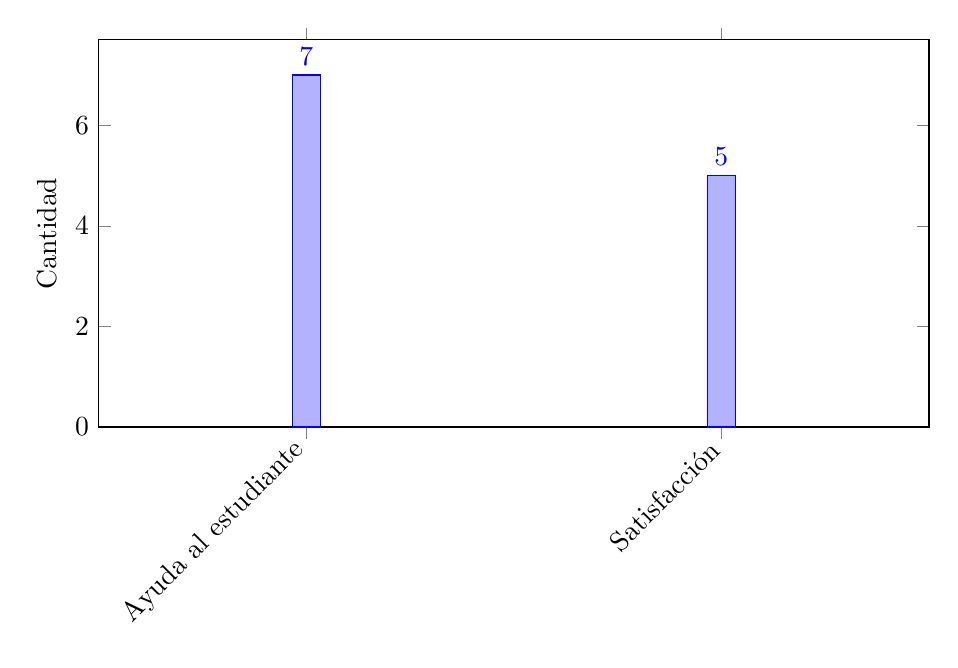
\begin{tikzpicture}
				\begin{axis}[
					ybar,
					width=\textwidth,
					height=6.5cm,
					symbolic x coords={Ayuda al estudiante, Satisfacción},
					xtick=data,
					ylabel={Cantidad},
					ymin=0,
					nodes near coords,
					enlarge x limits=0.5,
					x tick label style={rotate=45, anchor=east}
					]
					\addplot coordinates {(Ayuda al estudiante, 7) (Satisfacción, 5)};
				\end{axis}
			\end{tikzpicture}
			\subcaption{Alertas sonoras y luminosas del sistema.}
			\label{fig:SoundAndLigth}
		\end{minipage}
		\begin{minipage}{0.45\textwidth}
			\centering
			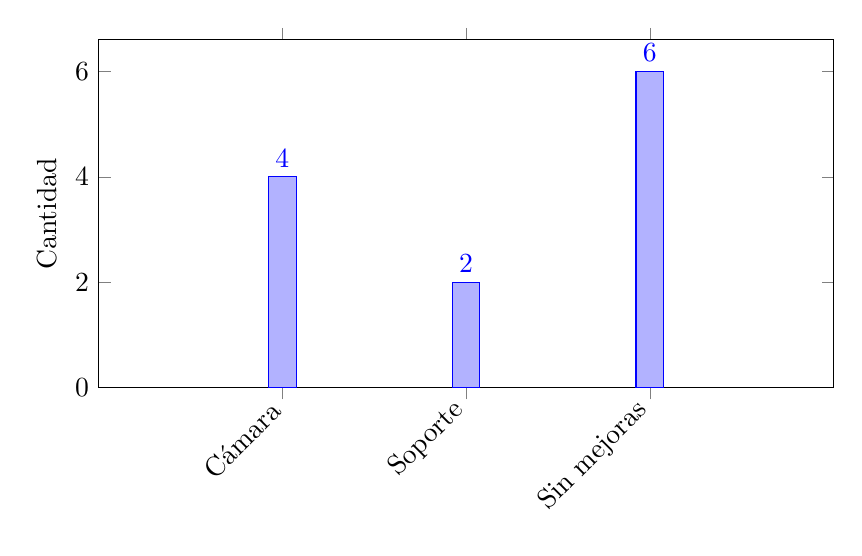
\begin{tikzpicture}
				\begin{axis}[
					ybar,
					height=6cm,
					width=0.9\textwidth,
					symbolic x coords={Cámara, Soporte, Sin mejoras},
					xtick=data,
					ylabel={Cantidad},
					ymin=0,
					nodes near coords,
					enlarge x limits=0.5,
					x tick label style={rotate=45, anchor=east}
					]
					\addplot coordinates {(Cámara, 4) (Soporte, 2) (Sin mejoras, 6)};
				\end{axis}
			\end{tikzpicture}
			\subcaption{Sugerencias para mejorar el sistema.}
			\label{fig:Improvements}
		\end{minipage}
		\begin{minipage}{0.45\textwidth}
			\centering
			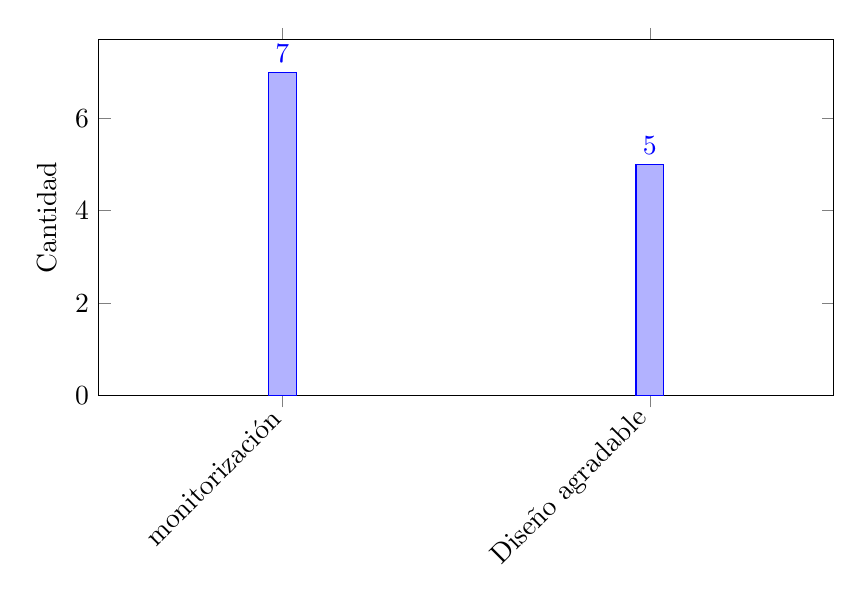
\begin{tikzpicture}
				\begin{axis}[
					ybar,
					height=6.1cm,
					width=0.9\textwidth,
					symbolic x coords={monitorización, Diseño agradable},
					xtick=data,
					ylabel={Cantidad},
					ymin=0,
					nodes near coords,
					enlarge x limits=0.5,
					x tick label style={rotate=45, anchor=east}
					]
					\addplot coordinates {(monitorización, 7) (Diseño agradable, 5)};
				\end{axis}
			\end{tikzpicture}
			\subcaption{Razones para recomendar el sistema.}
			\label{fig:ReasonsRecomend}
		\end{minipage}
		\caption{Resultados de preguntas realizadas a los padres sobre el proceso de monitorización de sus hijos de primaria usando Torddis mientras hacen sus tareas.}
		\label{fig:AnswerOfOpenQuestion}
	\end{figure}
	
	En las preguntas 3 ("¿Le gusta el diseño de la aplicación móvil Torddis? ¿Por qué?"), 4 ("¿Es adecuada la forma en que se visualizan los datos de monitorización de distracción de su hijo en la aplicación móvil Torddis? ¿Por qué?"), 5 ("¿Cree que este sistema ayudaría a mejorar la concentración de su hijo y mantenerlo informado mientras realiza sus tareas escolares? ¿Por qué?"), y 7 ("¿Estaría dispuesto a seguir usando el sistema Torddis?"), todos los tutores expresaron comentarios positivos. Manifestaron que les agrada el diseño de las vistas de la aplicación móvil, destacaron la organización de los datos históricos y los gráficos de informes, confirmaron que el sistema prototipo apoya eficazmente la concentración de los niños manteniéndolos informados cuando el niño se distrae, e indicaron su disposición a continuar usando el sistema Torddis.
	
	La pregunta 6 tenía como objetivo recopilar información sobre las mejoras que se podrían hacer a Torddis. Los comentarios obtenidos incluyen el uso de una cámara de mayor calidad y la mejora del soporte en el que se monta la cámara. Sin embargo, un alto porcentaje de usuarios mencionó que el dispositivo no necesita más mejoras. Estos resultados se muestran en la Figura \ref{fig:Improvements}. Por su parte, la pregunta 8 recopiló las razones por las que los evaluadores de Torddis recomendarían el uso de este sistema para la monitorización de estudiantes durante sus actividades escolares. La Figura \ref{fig:ReasonsRecomend} muestra las razones mencionadas por los tutores, incluyendo que les ayuda en la monitorización de sus estudiantes y su diseño agradable.
	
	\section{Conclusiones}
	\label{seccion:Seis}
	El sistema prototipo Torddis ha demostrado ser una herramienta efectiva y bien recibida para la monitorización y mejora de la concentración de los estudiantes durante sus actividades escolares. Las evaluaciones, que incluyen pruebas funcionales y cuestionarios de usabilidad, revelaron que el sistema cumple con los requisitos técnicos esperados y es altamente valorado por los usuarios finales, es decir, los tutores.
	
	El análisis de los datos demográficos y de monitorización indica que Torddis tiene un impacto significativo en la gestión de la distracción de los niños, proporcionando a los tutores una herramienta valiosa para mantener a los estudiantes enfocados en sus tareas. La alta puntuación en el cuestionario de usabilidad SUS refuerza la percepción de que el sistema es fácil de usar y efectivo en su propósito.
	
	El sistema de reconocimiento de personas de Torddis es eficiente, con una tasa de éxito del 92.86\% y un tiempo promedio de reconocimiento de aproximadamente 0.81 segundos, demostrando un sólido desempeño en condiciones de prueba. Del mismo modo, el sistema de reconocimiento de expresiones faciales muestra una tasa de éxito del 92.86\% con un tiempo promedio de reconocimiento de aproximadamente 1.36 segundos, destacando por sus tiempos de respuesta rápidos y su fiabilidad. El sistema de reconocimiento de la presencia de sueño es razonablemente eficiente, alcanzando una tasa de éxito del 85.71\% y un tiempo promedio de reconocimiento de aproximadamente 3.43 segundos, lo que indica un rendimiento adecuado.
	
	El sistema de reconocimiento de objetos distractores, con una tasa de éxito del 78.57\% y un tiempo promedio de reconocimiento de aproximadamente 2.33 segundos, funciona adecuadamente en condiciones de prueba.
	
	Además, los comentarios de las preguntas abiertas muestran un fuerte respaldo al diseño y funcionalidad del sistema, con valiosas sugerencias para futuros desarrollos. Los tutores destacaron la importancia de las alertas visuales y auditivas para mantener a los estudiantes alertas y la conveniencia de las opciones de configuración y monitorización del sistema.
	
	En conclusión, Torddis ha superado las expectativas en términos de funcionalidad y usabilidad, demostrando ser una solución viable y efectiva para mantener la concentración de los estudiantes en entornos de aprendizaje. El éxito de este proyecto subraya la importancia de la innovación tecnológica en la educación y sienta las bases para futuras mejoras y expansiones del sistema.
	
	\section*{Agradecimientos}
	
	Este trabajo de investigación ha sido financiado por la subvención PID2022-139297OB-I00, financiada por MICIU/AEI/10.13039/501100011033 y por el FEDER/UE.
	
	\printcredits
	
	\bibliographystyle{cas-model2-names}
	
	% Loading bibliography database
	\bibliography{torddisC&E-refs}
	
	\clearpage
	
	\appendix
	\section{Consentimiento Informado} \label{Appendix:InformedConsent}
	Estimado Participante,
	
	El propósito de este documento es proporcionarle la información necesaria para decidir si desea o no participar en el proyecto titulado "Sistema basado en Internet de las Cosas para monitorizar la distracción de niños durante sus actividades académicas en casa", realizado bajo la dirección del Profesor Gleiston Cicerón Guerrero Ulloa MDS.
	
	La participación implica el uso del sistema proporcionado, siguiendo las instrucciones de los investigadores. Se le pedirá que se siente en un lugar específico para utilizar una aplicación móvil. Mientras tanto, su hijo será monitoreado por un dispositivo inteligente llamado "Torddis" mientras realiza una tarea específica dirigida por los investigadores. El tiempo de participación es de aproximadamente 30 minutos, dependiendo de cada participante. Estas actividades se realizarán en una de las casas de los investigadores.
	
	La información obtenida a través de este estudio se mantendrá estrictamente confidencial y sus nombres no serán utilizados. Usted tiene el derecho de retirar el consentimiento para participar en cualquier momento. El estudio no implica ningún riesgo para usted, ni recibirá compensación alguna. Si tiene alguna pregunta sobre este proyecto, puede contactarnos en gguerrero@uteq.edu.ec.
	
	\vspace{0.5cm}
	\noindent\rule{3.65cm}{0.4pt} \hspace{1.1cm} \rule{4cm}{0.4pt} \hspace{1.1cm} \rule{4.2cm}{0.4pt}\\
	Carlos Almeida-Dueñas \hspace{2cm} John Plazarte-Suárez \hspace{2cm} Gleiston Guerrero-Ulloa
	
	Después de leer el procedimiento descrito anteriormente, de que los investigadores le expliquen el procedimiento y de responder a cualquier pregunta, el participante (firmante) da voluntariamente su consentimiento para participar en este estudio.
	
	\vspace{0.5cm}
	\noindent
	Participante: \_\_\_\_\_\_\_\_\_\_\_\_\_\_\_\_\_\_\_\_\_\_\_\_\_\_\_\_\_\_\_\_\_\_\_\_
	Firma: \_\_\_\_\_\_\_\_\_\_\_\_\_\_\_\_\_\_\_\_\_\_\_\_
	Fecha: \_\_\_\_\_\_\_\_\_\_
	
	\clearpage
	\section[\appendixname~\thesection]{Encuesta Demográfica} \label{Appendix:DemographicSurvey}
	\vspace{12pt}
	\noindent
	\textbf{1. Nombre Completo: \_\_\_\_\_\_\_\_\_\_\_\_\_\_\_\_\_\_\_\_\_\_\_\_\_\_\_\_\_\_\_\_\_\_\_\_\_\_\_\_\_\_\_\_\_}
	
	\vspace{12pt}
	\noindent
	\textbf{2. Edad: \_\_\_\_\_\_\_\_\_\_}
	
	\vspace{12pt}
	\noindent				
	\textbf{3. Nivel de Educación:}
	
	\begin{itemize}
		\item Sin educación ( )
		\item Primaria ( )
		\item Secundaria ( )
		\item Superior ( )
	\end{itemize}
	
	\noindent
	\textbf{4. Género:}
	
	\begin{itemize}
		\item Masculino ( )
		\item Femenino ( )
		\item Otro ( )
	\end{itemize}
	
	%\vspace{12pt.}
	\noindent
	\textbf{5. ¿Cómo ha sido su experiencia como padre en monitorizar las distracciones de su hijo mientras realiza sus tareas escolares?}
	
	\begin{itemize}
		\item Fácil ( )
		\item Regular ( )
		\item Compleja ( )
		\item Muy compleja ( )
	\end{itemize}
	
	%\vspace{12pt.}
	\noindent
	\textbf{6. ¿Con qué frecuencia monitoriza las actividades escolares de su hijo?}
	
	\begin{itemize}
		\item Nunca ( )
		\item A veces ( )
		\item Casi siempre ( )
		\item Siempre ( )
	\end{itemize}
	
	%\vspace{12pt.}
	\noindent
	\textbf{7. ¿Qué estrategias ha implementado para mejorar la concentración de su hijo durante sus tareas escolares?}
	
	\vspace{12pt}
	\noindent
	\rule{\textwidth}{1pt}
	
	\vspace{12pt}
	\noindent
	\rule{\textwidth}{1pt}
	
	\clearpage
	\section[\appendixname~\thesection]{Cuestionario SUS}
	\label{Appendix:SUSQuestionarie}
	
	
	\subsection[\appendixname~\thesection]{Cuestionario en Escala Likert}
	\label{Appendix:LikertScale}
	Las preguntas del cuestionario SUS usando la escala Likert se muestran en la Tabla \ref{tab:SUSQuestion}.
	
	\begin{table}[bt!]
		\caption{Cuestionario SUS \label{tab:SUSQuestion}}
		\centering
		\begin{tabular}{|p{10cm}|c|c|c|c|c|}
			\hline
			\textbf{Preguntas} & 1 & 2 & 3 & 4 & 5 \\
			\hline
			1. Me gustaría utilizar el sistema Torddis frecuentemente. & & & & & \\
			\hline
			2. Encontré el sistema innecesariamente complejo. & & & & & \\
			\hline
			3. Pensé que el sistema era fácil de usar. & & & & & \\
			\hline
			4. Necesitaría el apoyo de un técnico/profesor para usar el sistema. & & & & & \\
			\hline
			5. Encontré que las diversas funciones del sistema estaban bien integradas (constituían un todo). & & & & & \\
			\hline
			6. Pensé que había demasiadas inconsistencias en el sistema. & & & & & \\
			\hline
			7. Me imagino que la mayoría de las personas aprenderían a usar el sistema rápidamente. & & & & & \\
			\hline
			8. Encontré el sistema muy difícil de usar. & & & & & \\
			\hline
			9. Me sentí muy seguro/cómodo usando el sistema. & & & & & \\
			\hline
			10. Necesito aprender muchas cosas antes de poder usar el sistema. & & & & & \\
			\hline
		\end{tabular}
	\end{table}
	
	\subsection[\appendixname~\thesection]{Preguntas Abiertas del Cuestionario SUS}
	\label{Appendix:OpenQuestions}
	Las preguntas abiertas del cuestionario SUS se muestran en la Tabla \ref{tab:OpenQuestion}.
	\begin{table}[bt!]
		\centering
		\caption{Preguntas Abiertas del Cuestionario SUS \label{tab:OpenQuestion}}
		\begin{tabularx}{\textwidth}{c X }
			\toprule
			\textbf{No.} & \textbf{Pregunta} \\
			\midrule
			1 & En general, ¿cuál es su opinión sobre el sistema? \\
			2 & ¿Le gustaron los sonidos y/o luces que contiene el dispositivo Torddis? Por favor responda sí o no, y proporcione la razón. \\
			3 & ¿Le gustó el diseño de la pantalla de la aplicación móvil de Torddis? Por favor responda sí o no, y proporcione la razón. \\
			4 & ¿Le parece adecuada la forma en que se visualizan los datos de monitorización de distracción de su hijo en la aplicación móvil Torddis? Por favor responda sí o no, y proporcione sugerencias. \\
			5 & ¿Cree que este sistema ayudaría a mejorar la concentración de su hijo y a mantenerle informado cuando esté distraído? Por favor responda sí o no, y proporcione la razón. \\
			6 & ¿Cree que hay algo que debería mejorarse en el sistema Torddis (Dispositivo y Aplicación Móvil)? En caso afirmativo, ¿qué? \\
			7 & ¿Estaría dispuesto a continuar usando el sistema Torddis? Por favor responda sí o no, y proporcione la razón. \\
			8 & ¿Recomendaría este sistema a otras personas interesadas en monitorizar la distracción de niños mientras realizan tareas escolares? Por favor responda sí o no, y proporcione la razón. \\ \bottomrule
		\end{tabularx}
	\end{table}
\end{document}

